%%%% IACR Transactions TEMPLATE %%%%
% This file shows how to use the iacrtrans class to write a paper.
% Written by Gaetan Leurent gaetan.leurent@inria.fr (2020)
% Public Domain (CC0)

%%%% 1. DOCUMENTCLASS %%%%
%\documentclass[journal=tosc,final]{iacrtrans}
\documentclass[article]{iacrtrans}

\newcommand{\gurgen}[1]{{\color{brown} [Gurgen: #1]}}
\newcommand{\andreea}[1]{{\color{blue} [Andreea: #1]}}
\newcommand{\daria}[1]{{\color{violet} [Daria: #1]}}
\newcommand{\valentina}[1]{{\color{orange} [Valentina: #1]}}
\newcommand{\ahmad}[1]{{\color{purple} [Ahmad: #1]}}

\usepackage{algorithm}
\usepackage{listings}
\usepackage{array} 
\usepackage{longtable} 
\usepackage{adjustbox}
\usepackage{algorithmicx}
\usepackage[width=0.8\textwidth]{caption}
\captionsetup[figure]{labelfont=bf} 
\usepackage{float} % For [H] positioning
\usepackage{placeins} % For \FloatBarrier
\usepackage{listings}
\usepackage{tikz}
\usepackage{graphicx} 
\usepackage{subcaption}
\usepackage{indentfirst}


\usepackage[noend]{algpseudocode}
\usepackage{tablefootnote}
\usepackage{tabularx}
\usepackage{adjustbox}

\usepackage{authblk}

\usepackage{xcolor}
\lstset{
  basicstyle=\ttfamily\small,
  breaklines=true,
  breakatwhitespace=false,
  columns=fullflexible,
  frame=single,
  backgroundcolor=\color{gray!10},
  keywordstyle=\color{blue},
  showstringspaces=false
}

\setcounter{tocdepth}{3}

\usepackage{fancyhdr} % Required for header control
\usepackage{etoolbox} % For list processing

% --- Define author names for headers ---
\makeatletter
% Extract raw author names without affiliations
\newcommand{\headerauthors}{%
  \begingroup
  \renewcommand{\and}{, } % Replace "\and" with commas
  \renewcommand{\AB@affillist}{} % Ignore affiliations
  % \@author % Raw author names
  
  \endgroup
}
\makeatother

% --- Configure headers ---
\pagestyle{fancy}
\fancyhf{} % Clear all headers/footers
\fancyhead[C]{\headerauthors} % Authors in center header
\fancyfoot[C]{\thepage} % Page number in footer

%%%% NOTES:
% - Change "journal=tosc" to "journal=tches" if needed
% - Change "submission" to "final" for final version
% - Add "spthm" for LNCS-like theorems

%%%% 2. PACKAGES %%%%
% \usepackage{lipsum} % Example package -- can be removed
\title{FHERMA Cookbook: FHE Components for Privacy-Preserving Applications}
% %%%% 3. AUTHOR, INSTITUTE %%%%
\author[1]{Janis Adamek}
\author[2]{Aikata Aikata}
\author[3]{Ahmad Al Badawi}
\author[3]{Andreea Alexandru}
\author[4]{Armen Arakelov}
\author[4]{Gurgen Arakelov}
\author[1]{Philipp Binfet}
\author[5]{Victor Correa}
\author[6]{Jules Dumezy}
\author[4]{Sergey Gomenyuk}
\author[4]{Valentina Kononova}
\author[5]{Dmitrii Lekomtsev}
\author[7]{Vivian Maloney}
\author[8]{Chi-Hieu Nguyen}
\author[3]{Yuriy Polyakov}
\author[4]{Daria Pianykh}
\author[9]{Hayim Shaul}
\author[1]{Moritz Schulze Darup}
\author[1]{Dieter Teichrib}
\author[5]{Dmitry Tronin}

\affil[1]{TU Dortmund University, Germany}
\affil[2]{Graz University of Technology, Austria}
\affil[3]{Duality Technologies, USA}
\affil[4]{Fair Math, USA}
\affil[5]{Independent Researcher}
\affil[6]{Université Paris-Saclay, CEA, List, F-91120, Palaiseau, France}
\affil[7]{Johns Hopkins University Applied Physics Laboratory, USA}
\affil[8]{University of Technology Sydney, Australia}
\affil[9]{IBM Research}

% \affil[5]{Control and Cyberphysical Systems Group, TU Dortmund University, Germany}

% \affil[7]{Université Paris-Saclay, CEA, List, France}




\date{Version 0.171} 



%%%% NOTES:
% - We need a city name for indexation purpose, even if it is redundant
%   (eg: University of Atlantis, Atlantis, Atlantis)
% - \inst{} can be omitted if there is a single institute,
%   or exactly one institute per author

%%%% 4. TITLE %%%%
% \title{FHERMA Cookbook: Foundational Components for Privacy-Preserving Computation}
%%%% NOTES:
% - If the title is too long, or includes special macro, please
%   provide a "running title" as optional argument: \title[Short]{Long}
% - You can provide an optional subtitle with \subtitle.
\usepackage[backend=bibtex]{biblatex} 
\addbibresource{biblio.bib} 

\begin{document}
\institute{}
\maketitle

\thispagestyle{plain} 

%%%% 5. KEYWORDS %%%%
\keywords{fhe, challenges, cryptography, privacy, fhe-computer, encryption, library, fherma}


%%%% 6. ABSTRACT %%%%
\begin{abstract}
Fully Homomorphic Encryption (FHE) enables computation over encrypted data and is considered a fundamental tool for privacy-preserving systems. Despite significant theoretical progress, its practical adoption remains limited. One contributing factor is the absence of reusable, application-level components suitable for integration into real-world systems.

This work introduces a library of FHE components developed through a competition-based framework. The components are outcomes of a series of formalized challenges published on the FHERMA platform, each targeting a specific challenge—such as comparison, sorting, or matrix operations—under concrete cryptographic and performance constraints.


This initial release includes contributions from independent researchers and reflects a variety of approaches across different FHE schemes. The library is intended to expand over time as new challenges are introduced and solved, forming a foundation for building and evaluating privacy-preserving applications.
\end{abstract}

\newpage
\tableofcontents
\newpage
%%%% 7. PAPER CONTENT %%%%
\section{Introduction}

Fully Homomorphic Encryption (FHE) is a powerful cryptographic primitive that enables computations over encrypted data without access to the secret key. This capability has opened new frontiers in data privacy and security, making FHE particularly relevant in sensitive domains such as finance, healthcare, blockchain, and cloud computing. In machine learning (ML), for example, FHE enables the secure outsourcing of computation to untrusted environments while preserving the confidentiality of both data and models. It also plays a pivotal role in distributed and federated ML settings, supporting secure collaboration without data leakage \cite{cryptoeprint:2022/1602}. Similarly, in data analysis and blockchain, FHE enables privacy-preserving analytics and confidential smart contracts, respectively.

Despite significant advances in theory and implementation, the adoption of FHE at the application level remains limited. Several factors contribute to this gap. First, the development of FHE-based applications typically demands a high level of expertise in cryptography, numerical methods, and application-specific domains. Second, FHE operations are computationally intensive, often requiring substantial processing resources and optimization effort. Third, the field lacks standardized tools, benchmarks, and methodologies for building, testing, and comparing FHE-based software systems.

Among these challenges, one important limitation is the absence of an accessible library of high-level, reusable FHE components. Most existing FHE libraries expose only low-level primitives, requiring developers to construct even basic application logic from scratch. This significantly raises the barrier to entry and hinders the creation of robust, portable FHE applications.

To address this gap, we previously introduced the FHERMA platform \cite{fherma:2024}, a community-driven initiative that formulates and hosts challenge problems designed to capture common application-level tasks in FHE. These challenges are organized across domains such as ML and blockchain, and contributors submit solutions that are automatically verified for correctness and performance. Accepted solutions form the basis of a modular, open-source library of FHE components.

In this paper, we present the first public release of the FHERMA FHE Components Library, a curated collection of verified solutions to the initial FHERMA challenges. Each component in the library addresses a concrete task (e.g., comparison, sorting, matrix operations) under strict cryptographic and efficiency constraints. The components are designed to be composable and interoperable, enabling developers to rapidly prototype privacy-preserving applications without deep knowledge of FHE internals.

The library is intended to evolve over time as new challenges are posed and solved. Our long-term vision is to develop a living, community-maintained resource that accelerates the adoption of FHE by reducing technical barriers and establishing a foundation for standardized development practices. This document will be continuously expanded to reflect contributions from across the FHE ecosystem.



\subsection{Overview of FHE Capabilities}

Fully Homomorphic Encryption (FHE) enables arbitrary computations on encrypted data without revealing the underlying plaintext. This cryptographic primitive has emerged as a foundational building block for privacy-preserving technologies, offering the ability to process sensitive information without compromising confidentiality.

Modern FHE schemes fall into three main categories, distinguished by the arithmetic they support:

\begin{itemize}
    \item \textbf{Integer arithmetic schemes}, such as BGV~\cite{bgv:2011/277} and BFV~\cite{bfv:2012/144, bra12:2012/078}, operate over modular integer rings and are particularly suited for applications that require exact computations over vectors, including private statistics and secure voting protocols.
    
    \item \textbf{Boolean circuit schemes}, including DM~\cite{dm:2014/816} and CGGI~\cite{cggi:2016/870}, focus on evaluating logic circuits and decision diagrams. These schemes often offer fast bootstrapping and compact ciphertexts but have a limited support for Single Instruction Multiple Data (SIMD)-style batch processing. Note that these schemes can also support small integers.

    \item \textbf{Approximate arithmetic schemes}, such as CKKS~\cite{ckks:2016/421}, support computations on real- and complex-valued vectors with bounded precision. This class is particularly effective for implementing machine learning inference, signal processing, and other numerical tasks in an encrypted domain.
\end{itemize}

The most widely used schemes rely on the Learning With Errors (LWE) or Ring-LWE hardness assumptions for security. A fundamental constraint across all classes is the presence of noise that accumulates with each encrypted operation. Bootstrapping, a mechanism for noise management, enables unbounded computation but introduces significant overhead. As a result, performance constraints—especially multiplicative depth—continue to influence how FHE applications are designed.

\subsection{Application-Level Challenges }

Despite significant advances in the theory and implementation of Fully Homomorphic Encryption (FHE), the development of real-world applications remains a challenging task. One of the primary obstacles is the substantial gap between cryptographic libraries and the needs of application developers. Most libraries provide access to low-level primitives—such as ciphertext arithmetic and key management—without offering abstractions suitable for expressing higher-level computational logic.

As a result, developers must construct even basic operations, such as comparisons or control flow, manually using low-level tools. This often involves managing scheme-specific constraints like ciphertext noise, multiplicative depth, level consumption, and data packing. The lack of abstraction not only increases the cognitive and engineering burden but also leads to redundant implementations, non-portable code, and a higher likelihood of subtle errors or inefficiencies.

In schemes such as CKKS, additional complexity arises from approximate computation. Developers must balance trade-offs between accuracy, circuit depth, and performance—frequently relying on advanced techniques such as polynomial approximations, rescaling heuristics, and bootstrapping strategies. These challenges become more pronounced in applications involving complex logic or large data flows, such as private machine learning or secure data aggregation.

Altogether, the absence of well-established methods for expressing and composing functionality at the application level limits the scalability, maintainability, and adoption of FHE technologies. Bridging this gap is critical for enabling the development of secure and privacy-preserving applications that are both practical and trustworthy.


\subsection{A modular component library for application layer}

A major challenge in FHE application development is the lack of abstraction layers that separate algorithmic logic from scheme-specific cryptographic details. Developers must translate high-level tasks into low-level operations while managing constraints such as noise growth, ciphertext levels, and packing formats. This not only increases the risk of error but also discourages modularity, reuse, and experimentation.

To address this, we propose a modular FHE component library designed to sit at the intermediate FHE Components layer --- between low-level cryptographic operations and high-level compilers or user-facing APIs. The layered design is depicted in Figure \ref{fig:fhe_layers}. 

        \begin{figure}[H]
            \centering
            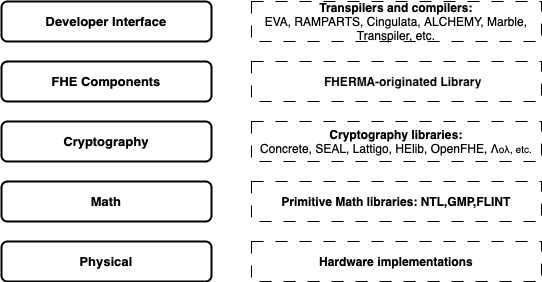
\includegraphics[width=0.7\textwidth]{fhe_layers.png}
            \caption{Multi-layer design of FHE development environment
}
            \label{fig:fhe_layers}
        \end{figure}

This idea aligns with the layered ecosystem design presented in \cite{openfhe:2022/915} and implemented in OpenFHE library, where cryptographic, arithmetic, and application logic are separated into distinct layers to promote standardization and reusability.

In this design:

\begin{itemize}
    \item The \textbf{Cryptography layer} handles scheme-specific details such as key management, encryption/decryption, bootstrapping, and noise tracking.
    \item The \textbf{FHE Components layer} defines modular building blocks such as encrypted comparison, ReLU, matrix multiplication, or sorting. These components are designed to be reusable and portable across FHE schemes.
    \item The \textbf{Developer Interface layer} integrates these components into compilers or DSLs (e.g., HEIR, EVA), exposing high-level APIs to application developers.
\end{itemize}

This structure will allow users to write applications in terms of abstract functions, while the system handles cryptographic translation and optimization.

In Section~\ref{components} of this paper, we present a curated selection of FHE components developed and submitted through the FHERMA challenges platform. These components span both elementary and compound operations, reflecting current priorities and challenges in encrypted computation.

\iffalse
\andreea{I think it would be valuable to have section showing how to concretely use these components from the library in a larger application (the code for it). This would underline the usability of the component library.}
\valentina{The usage of the fundamental components are partially shown in different challenge solutions, but participants usually make their own approximations. I believe the code of usage should be demonstrated in the polycircuit repository. But I agree that we can work on it and add this section in the following versions of the cookbook. }
\andreea{With my comment, I wanted to address this wishlist item from above ``standardized, reusable FHE components”. We need to make explicit how we envision the components being reused in the context of larger applications (not just evaluating the component). There should be a section on the polycircuit library to show the concrete usage and demonstrate the repeated usefulness.}
\fi

\subsection{Objectives and Design Considerations}
To make the structure explained in the section above usable in practice, our goal is to enable application developers to express computations entirely at the level of abstract reusable components, without manually managing encryption parameters, noise growth, or bootstrapping. The component library is designed for integration into higher-level toolchains and DSLs, allowing FHE applications to be written in a modular and declarative style.

For example, a  neural network for privacy-preserving inference can be expressed over encrypted inputs using a standard activation component from the library. As shown in Listing \ref{lst:neuron}, the developer works with encrypted types and high-level logic (\verb|relu|), while the compiler and backend resolve the component call into a concrete FHE circuit.

\vspace{0.5em}
\begin{lstlisting}[language=Rust, caption={Encrypted neuron with ReLU activation}, label={lst:neuron}]
fn neuron(inputs: [secret<i32>; N], weights: [secret<i32>; N], bias: secret<i32>) -> secret<i32> {
let mut acc = bias;
for i in 0..N {
acc = acc + inputs[i] * weights[i];
}
return polycircuit::relu(acc);
}
\end{lstlisting}
\vspace{0.5em}

This style of usage illustrates the long-term objective of the library: to serve not only as a set of benchmarkable components, but as the foundation for high-level programming with encrypted data. Components are intended to be reused and composed within larger pipelines, such as machine learning inference or private analytics, without modifying their internal implementation.

To support this, the library will provide language-agnostic interfaces and is designed for integration with compiler frameworks such as HEIR, EVA, or custom MLIR-based compilers. Its role within the Component layer complements existing efforts at the Cryptography and Developer Interface levels, forming part of a full-stack FHE development ecosystem.


\section{Overview of the FHERMA Platform}

The \textbf{FHERMA platform} is designed to accelerate the development of practical Fully Homomorphic Encryption (FHE) applications by supporting the creation of an open-source library of reusable components. The platform provides a structured environment for evaluating FHE-based algorithms through formalized challenges. Its primary focus is on use cases in machine learning and blockchain, where FHE can offer strong privacy guarantees.

FHERMA supports both \emph{black box} and \emph{white box} challenges. In black box challenges, participants submit only the encrypted outputs of their algorithms; the platform evaluates these ciphertexts for correctness and efficiency without requiring access to the underlying implementation. This allows developers to preserve the confidentiality of their methods. In white box challenges, participants submit source code for performance evaluation in a confidential manner.

The platform supports multiple homomorphic encryption schemes, including CKKS\cite{ckks:2016/421}, BFV\cite{bfv:2012/144}, BGV\cite{bgv:2011/277}, DM/FHEW \cite{dm:2014/816}, and CGGI/TFHE\cite{cggi:2016/870} . In addition, it offers flexibility in cases where the most appropriate scheme is not obvious, allowing challenge designers to leave the choice of scheme to participants. 

FHERMA is compatible with a range of FHE libraries and toolkits, such as \texttt{OpenFHE}\cite{openfhe:2022/915}, \texttt{Lattigo}\cite{lattigo}, \texttt{HELayers}\cite{helayers}, and Apple’s FHE library. This broad compatibility enables participants to use their preferred development stacks.

Evaluation is performed in an automated and transparent manner. Solutions are tested against a comprehensive set of test cases, and rankings are updated in real time on a dynamic leaderboard. At the conclusion of each challenge, all encrypted inputs and secret keys are published, allowing independent verification of results.

The platform is continuously updated based on community feedback and ongoing research. It aims not only to address technical challenges but also to build a collaborative ecosystem. By engaging academic and industry contributors, FHERMA facilitates knowledge exchange and drives innovation in privacy-preserving computation.


\section{FHE Components Library }
The FHE Components Library is a structured collection of reusable building blocks designed to facilitate the development of applications based on fully homomorphic encryption (FHE). The library consists of a growing set of components, each encapsulating a specific operation or algorithmic primitive, implemented in a way that is compatible with practical FHE schemes.

To enhance clarity and reusability, the components are organized into functional groups. These include, for example, logical and bitwise operations, nonlinear approximations, linear algebra routines, and data manipulation primitives. This modular structure is intended to reflect the recurring patterns found in privacy-preserving computations and to support the composition of complex algorithms from verified, well-understood parts.

The library is released under a permissive open-source license, with the goal of supporting the broad adoption and practical deployment of FHE-based solutions. By providing standard, tested implementations of common computational tasks, the FHE Components Library aims to lower the entry barrier for developers, reduce duplication of effort, and enable a more rapid translation of theoretical advances in homomorphic encryption into usable software systems.

The components are intended to be extensible and adaptable to different FHE backends and parameter settings, and contributions from the community are actively encouraged.

Each of these components, when described independently, specifies some concrete encryption parameters. Nevertheless, in the context of a larger application, different parameters (under some restrictions) can be used.
% \andreea{Question: in the library of components, will parameters such as the number of slots be given as arguments or fixed to $2^{12}$?}\\
% \daria{Answer: no, parameters are not gonna be fixed. There will be some restrictions, however}

\label{components}
\label{sec:component_list}
\subsection{Logical and Bitwise Operations}
\subsubsection{Sign}
This component calculates the sign elementwise on an encrypted vector of real numbers, using the OpenFHE library. The goal is to take an encrypted input vector $A = [x_1, \ldots, x_n]$, where each $x_i \in [-1, 1]$, and return an encrypted vector containing the sign of each element. In FHE schemes such as CKKS\cite{ckks:2016/421}, BGV\cite{bgv:2011/277}, BFV\cite{bfv:2012/144}, where discontinuous functions cannot be evaluated directly, polynomial approximations are essential for comparison and max-pooling operations in privacy-preserving ML. 

\paragraph{Specification}

 \begin{itemize}
    \item \textbf{Input}: 
        \begin{itemize}
            \item single packed ciphertext containing the input vector of $2^{12}$ slots
            \item cryptocontext
            \item public key
            \item multiplication key
        \end{itemize}
    \item \textbf{Output}
        \begin{itemize}
            \item encrypted vector sign(x)
        \end{itemize}
    \item \textbf{Encryption parameters}:
        \begin{itemize}
            \item Number of slots: $2^{12}=4096$ 
            \item Multiplication depth: 10
            \item Fractional part precision (ScaleModSize): 50 bits
        \end{itemize}

\end{itemize}


\paragraph{Algorithm overview}\mbox{}\\

Since the sign function is not polynomial, it should be approximated by Chebyshev polynomials to tailor it to encrypted arithmetic operations. The greater the degree of the polynomial, the more accurate the approximation, but the degree is limited by the multiplicative depth.\\


\textbf{Series Evaluation}. A multiplicative depth of 10 allows the Chebyshev series to be evaluated only up to the $1026$-th coefficient. So, a first step is to precalculate the first 1026 coefficients:
\[ \texttt{coeff\_1026 = numpy.polynomial.chebyshev.chebinterpolate(numpy.sign,1026)} \]

The accuracy of a polynomial approximation is rigorously evaluated by its ability to replicate the true function’s behavior over a specified domain. 
In this context, accuracy is quantified by comparing the polynomial's predictions against a validation dataset, typically measured by the percentage of correctly predicted signs (positive or negative) of the function's output. The accuracy of this polynomial is $99.96\%$, meaning it correctly predicts the sign of the output in $99.96\%$ of the validation test cases. \\
% \andreea{I understand that this accuracy refers to how many signs were computed correctly on a validation vector, and many examples use this accuracy as a justification for the solution, but this should be described before.}\\
% \daria{Added brief description of accuracy}


\textbf{Depth Optimization via Recursion}. High-degree Chebyshev terms are recursively broken down using the identity:
    \[
        T_m = 2 \cdot T_i \cdot T_j - T_k
    \]
    until intermediate terms can be safely multiplied at reduced depth.  \\
    For example, for $T_{1009}$:
\begin{align}
    \text{c}\times T_{1009} &&\rightarrow&& \text{2c}\times T_{512}\times T_{497}-\text{c}\times T_{15} && \rightarrow &&   T_{512}\times(\text{2c}\times T_{497})-\text{c}\times T_{15}\\
    \text{2c}\times T_{497} && \rightarrow &&  \text{4c}\times T_{256}\times T_{241}-\text{2c}\times T_{15} && \rightarrow  &&  T_{256}\times(\text{4c}\times T_{241})-\text{2c}\times T_{15}\\
    \text{4c}\times T_{241} && \rightarrow  && \text{8c}\times T_{128}\times T_{113}-\text{4c}\times T_{15} && \rightarrow &&   T_{128}\times(\text{8c}\times T_{113})-\text{4c}\times T_{15}\\
    \text{8c}\times T_{113} && \rightarrow &&  \text{16c}\times T_{64}\times T_{49}-\text{8c}\times T_{15} && \rightarrow &&   T_{64}\times(\text{16c}\times T_{49})-\text{8c}\times T_{15}\\
    \text{16c}\times T_{49} && \rightarrow &&  \text{32c}\times T_{32}\times T_{17}-\text{16c}\times T_{15} && \rightarrow &&   T_{32}\times(\text{32c}\times T_{17})-\text{16c}\times T_{15}\\
    \text{32c}\times T_{17} && \rightarrow &&  \text{64c}\times T_{16}\times T_{1}-\text{32c}\times T_{15} && \rightarrow &&   T_{16}\times(\text{64c}\times T_{1})-\text{32c}\times T_{15}
\end{align}
Upon the initial breakdown of ${T}_{1009}$, we observed that the series terms to be multiplied (${T}_{512}$, ${T}_{497}$) were at the same depth of nine. Unfortunately, this configuration made it impossible to perform a third multiplication with the coefficient ${c}$. Therefore, we recursively broke down the expression until we achieved terms (${T}_{16}$, ${T}_{1}$) at different depths (4,1). At this stage, we can multiply ${c}$ with ${T}_{1}$, bringing it to a depth of one. Subsequently, we can proceed to compute upwards the recursive breakdown to obtain $c \times {T}_{1009}$.\\

\textbf{Coefficient Pruning}. Since the sign function is an odd function, the even degree coefficients ($T_{2i}$) do not contribute to its approximation. Hence, only odd Chebyshev terms ($T_{2i+1}$) are evaluated.\\
    
\textbf{Polynomial Composition}. The same methodology is applied to evaluate all the remaining Chebyshev series coefficients - $T_{1011}$, $T_{1013}$, $T_{1015}$, $T_{1017}$, $T_{1019}$, $T_{1021}$, and $T_{1023}$. It is crucial to note that the recursion must be further broken down to evaluate higher degree coefficients. This additional evaluation increases accuracy from $99.96\%$ to $99.97\%$.\\

\textbf{Example Use Cases}

In general, having the ability of calculating sign means enabling comparison or max operations:
        \begin{align}
            \text{comp}(a,b) &= \frac{ \text{sign}(a-b)+1}{2}\\
            \text{max}(a,b) &= \frac{ (a+b)+(a-b) \text{sign}(a-b)}{2}
        \end{align}
        
In various applications in ML, the sign function serves as a foundational element for non-linear activation functions like the Rectified Linear Unit (ReLU) or Max Pooling. 




\subsubsection{Parity}
The function $\textsf{parity}(x)$ gets an integer and returns its least significant bit (LSB). In other words,
$\textsf{parity}(x)=x \bmod 2$, where $x \in \mathbb Z$.
 
\paragraph{Specification}

\begin{itemize}
    \item \textbf{Input}: 
        \begin{itemize}
            \item encrypted vector $x = (x_1, ... )$, where $x_i \in [0, 255]$
            \item cryptocontext
            \item public key
            \item multiplication key
        \end{itemize}
    \item \textbf{Output}
        \begin{itemize}
            \item an encrypted vector  $\textsf{parity}(x) = (\textsf{parity}(x_1), ... )$
        \end{itemize}
    \item \textbf{Encryption parameters}:
        \begin{itemize}
            \item Number of slots: $2^{16}$ 
            \item Multiplication depth: 29
            \item Fractional part precision (ScaleModSize): 59 bits
            \item First Module Size: 60 bits
        \end{itemize}
\end{itemize}    




\paragraph{Algorithm overview}\mbox{}\\

The core idea is to approximate the parity function $\textsf{parity}(x) = x \bmod 2$ using a trigonometric function with Chebyshev polynomials. Evaluating trigonometric functions in an encrypted domain is a well-established problem, which is frequently employed in the bootstrapping process to refresh the level count of an ``exhausted'' ciphertext \cite{Bossuat2021}. We refined this polynomial approximation using a modified Arnoldi method as introduced in \cite{Brubeck2021}.

\begin{enumerate}
    \item \textbf{Problem Transformation.} Convert the discrete parity function $\text{parity}(x) = x \mod 2$ to continuous domain through trigonometric formulation $f(x) = \frac{1}{2}(\cos(\pi(x+1)) + 1)$. Normalize input space using $y = \frac{x-128}{128}$ to work in $[-1,1]$, yielding transformed target $f(y) = \frac{1}{2}(\cos(128\pi y + \pi) + 1)$.
    \item \textbf{Initial Polynomial Approximation.} Approximate $\cos(\pi y + \frac{\pi}{128})$ using the 8th-degree Chebyshev polynomial $p(y)$ via \texttt{numpy.polyfit}.  Figure 1 shows an illustration of such approximation using a polynomial of degree 8.
        \begin{figure}[H]
            \centering
            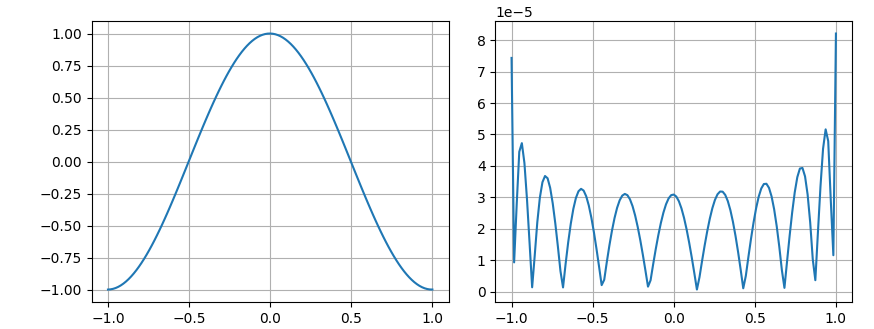
\includegraphics[width=0.8\textwidth]{parity_figures/parity_Figure_1.png}
            \caption{(left) Approximation of $cos(\pi y+ \frac{\pi}{128})$ using an 8th-degree polynomial. (right) Absolute error of the approximation.}
            \label{fig:parity-1}
        \end{figure}
    \FloatBarrier
    \item \textbf{Double-angle formula.} Now we have to apply double-angle formula $h(z) = 2z^2 - 1$ iteratively 7 times  to calculate $h^7 \circ p(y)$, which approximates $g(y) = \cos(128\pi y + \pi)$. But there is an initial maximum error of $>0.01$ observed at critical values (0, 126-128, 255-256).
       \begin{figure}[H]
            \centering
            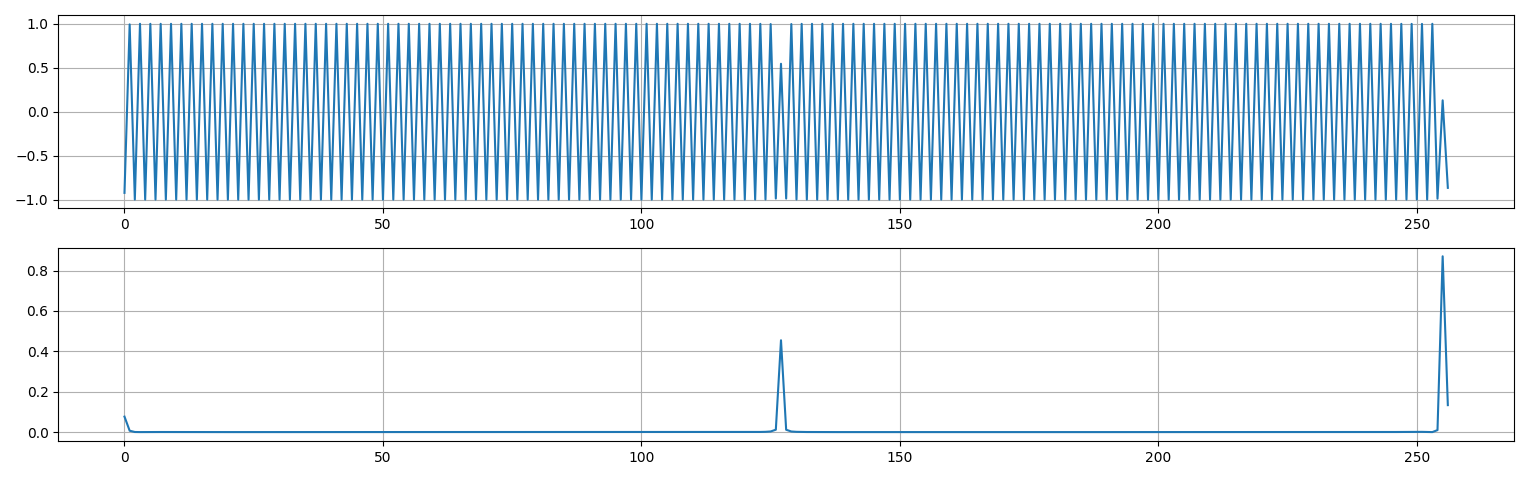
\includegraphics[width=0.8\textwidth]{parity_figures/parity_Figure_2.png}
            \caption{(top) Approximation of $\cos(128\pi y + \pi)$ after 7 double angle iterations. (bottom) Absolute error of the approximation.}
            \label{fig:parity-2}
        \end{figure}
    \item \textbf{Iterative Error Refinement.}
    To address this issue, we implemented a modified Arnoldi method [2] with weight updates: $w \leftarrow w \cdot |(h^7 \circ p)(y) - g(y)|$, where $g(y) = \cos(128\pi y + \pi)$. After 5 iterations, the maximum approximation error reduced to below $<3 \times 10^{-4}$ 
        \begin{figure}[H]
            \centering
            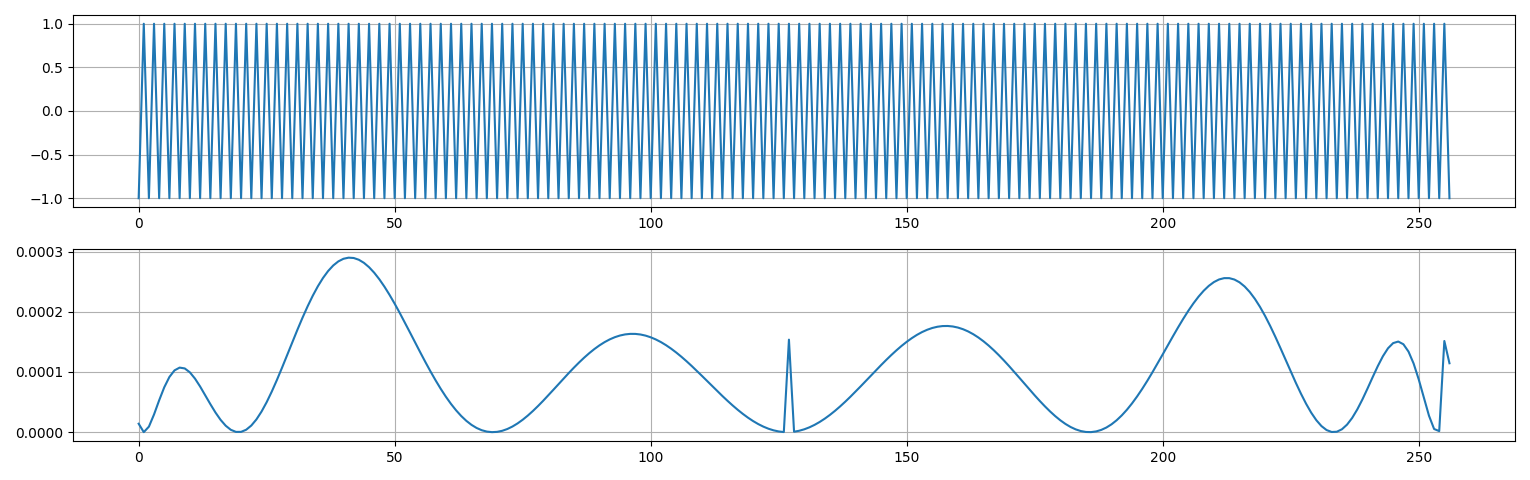
\includegraphics[width=0.8\textwidth]{parity_figures/parity_Figure_3.png}
            \caption{(top) The final approximation. (bottom) Absolute error of the approximation.}
            \label{fig:parity-3}
        \end{figure}
    \item \textbf{Symmetry Optimization.} Exploit even functions' property of $\cos(\pi y)$ to eliminate odd-degree terms in Chebyshev expansion. Obtain simplified coefficients:
    instead of directly approximating $\cos(\pi y + \frac{\pi}{128})$, we approximate $p(y)\approx cos(\pi y)$ using the same method and then evaluate $p(y + \frac{\pi}{128})$ ) to obtain $\cos(\pi y + \frac{\pi}{128})$. Since $\cos(\pi y )$ is an even function, its Chebyshev representation contains only even-degree terms, allowing us to omit the odd-degree terms for faster evaluation. The updated Chebyshev representation of $p$ is as follows.
        \begin{lstlisting}[breaklines=true, basicstyle=\ttfamily]
        [-0.3042513777371315, 0, -0.970882602838183, 0, 
         0.30291864798067064, 0, -0.02911740974995488, 0, 
         0.0013327077835582305]
        \end{lstlisting}

    \item \textbf{Coefficient Scaling.} Our target function is $f(y) = \frac{1}{2}(\cos(128\pi y + \pi) + 1)$, so the approximation of $\cos(128\pi y + \pi)$ must be scaled by $\frac{1}{2}$, which would incur an extra multiplication level. \\
    To avoid this, we scale the coefficients of $p$ by $a = \frac{2}{ \sqrt[2^7]{4}}$ to approximate $a \cos(\pi y)$. \\
    We then apply a series of transformations $h_i(y) = y^2 - 2 * (\frac{a}{2})^{2^i}$ to calculate $(h_7 \circ \cdots \circ h_1 \circ p)\left(y + \frac{\pi}{128}\right) \approx \frac{1}{2}\cos(128\pi y + \pi)$. \\
    \item \textbf{Final Composition.}
    The final approximation of $f(y)$ is obtained by adding $\frac{1}{2}$ to the resulting value. The multiplication depth of the whole computation is 12: 1 for evaluating $y$, 4 for evaluating $p(y)$ and 7 for the transformations $h_1, \ldots, h_7$.\\    
\end{enumerate}


\subsubsection{Shift}
The Shift Left (SHL) opcode in the Ethereum Virtual Machine (EVM) performs a bitwise shift left operation on an integer value. This operation is used to shift the bits of an integer to the left by a specified number of positions, effectively multiplying the number by $2^n$,  where $n$ is the number of positions shifted. 

\paragraph{Specification}
 \begin{itemize}
    \item \textbf{Input}: 
        \begin{itemize}
            \item encrypted value $x \in [0, 2^{16} - 1]$
            \item encrypted value $n \in [0, 16]$ is a number of shifted bits
            \item cryptocontext
            \item public key
            \item multiplication key
            \item rotation key for indexes [1, -1, 2, -2, 3, -3, 4, -4, 5, -5]
        \end{itemize}
    \item \textbf {Output}:
        \begin{itemize}
            \item The first slot should contain the value $y = \textsf{SHL}(x, n) = x << n $ which is equal to $x*2^n$.
        \end{itemize}
    \item \textbf{Encryption parameters}:
        \begin{itemize}
            \item Number of slots: $2^{16}$ 
            \item Multiplication depth: 29
            \item Fractional part precision (ScaleModSize): 59 bits
            \item First Module Size: 60 bits
            \item Bootstrapping: used
        \end{itemize}
\end{itemize}
    
\paragraph{Algorithm overview}\mbox{}\\
        
The proposed solution employs a two-way lookup table approach, using $x$ and $n$ as keys and $\textsf{SHL}(x, n)$ as the lookup value. In this way, the computation in the encrypted domain is expressed as:
\[
    \textsf{SHL}(c_x, c_n) = \sum_{i=0}^{2^{16} - 1} \left( \textsf{EQ}(c_x, i) \times \sum_{k=0}^{15} \textsf{EQ}(c_n, k) \times \textsf{SHL}(i, k) \right),
\]
where
\[
    \textsf{EQ}(a, b) = 
    \begin{cases} 
        1 & \text{if } a = b, \\
        0 & \text{if } a \neq b,
    \end{cases}
\]
is the equality function.

\begin{enumerate}  
    \item \textbf{Preprocessing (Performed Once)}. Generate a plaintext vector $p^{\text{in}} = [0, 1, \dots, 2^{16} - 1]$ representing all possible input values. For each shift amount $k \in [0, 15]$, precompute a plaintext vector $p_k^{\text{out}} = [\text{SHL}(0, k), \text{SHL}(1, k), \dots, \text{SHL}(2^{16} - 1, k)]$ containing the corresponding shifted outputs. Also generate a shift vector $p^{\text{shift}} = [0, 1, \dots, 15]$ to support shift amount comparisons.
    
    \item \textbf{Slot Duplication}. Replicate the encrypted values $c_x$ and $c_n$ across all slots to obtain $\text{Duplicate}(c_x)$ and $\text{Duplicate}(c_n)$, which have the original values copied into all $2^{16}$ slots.
    
    \item \textbf{Outer Equality Check (match x)}. Compute the ciphertext difference $c_{\text{diff}} = \text{Duplicate}(c_x) - p^{\text{in}}$, where $p^{\text{in}}$ is a plaintext encoding of all possible $x$ values.\\
    Raise $c_{\text{diff}}$ to the power $3 \cdot 2^{18}$ using Fermat’s Little Theorem to get $$c_{\text{eq\_x}} = 1 - c_{\text{diff}}^{3 \cdot 2^{18}},$$ which results in a ciphertext with 1 in the slot corresponding to $x$ and 0 elsewhere.
    
    \item \textbf{Inner Equality Check (match n)}. Compute the ciphertext difference $c_{\text{diff\_n}} = \text{Duplicate}(c_n) - p^{\text{shift}}$, where $p^{\text{shift}}$ is a plaintext vector encoding all shift amounts from 0 to 15.\\ 
    Evaluate a single Lagrange polynomial $p(z)$ over $c_{\text{diff\_n}}$ to get $c_{\text{eq\_n\_vec}} = p(c_{\text{diff\_n}})$, which yields a ciphertext vector with 1 in the slot corresponding to $n$ and 0 elsewhere.\\
    
    \item \textbf{Generate Masked Output}. For each $k \in [0, 15]$, extract the $k$-th slot value from $c_{\text{eq\_n\_vec}}$, broadcast it across all slots to get a mask ciphertext $\text{mask}_k$, and compute the product $\text{mask}_k \cdot p_k^{\text{out}}$.
    
    \item \textbf{Weighted Sum of Outputs}. Sum all products from previous step to get $c_{\text{sum}} = \sum_{k=0}^{15} \text{mask}_k \cdot p_k^{\text{out}}$, which holds the correct output in the slot indexed by $x$.
    
    \item \textbf{Apply Outer Equality Mask}. Multiply $c_{\text{eq\_x}}$ with $c_{\text{sum}}$ to isolate the result, and apply $\text{SumSlots}(\cdot)$ to move the correct value to the first slot.
    
    \item \textbf{Depth Optimization}. To avoid additional multiplicative depth, reorder the computation as $c_{\text{sum}} - c_{\text{diff}}^{2^{19}} \cdot (c_{\text{diff}}^{2^{18}} \cdot c_{\text{sum}})$, achieving the same result with total depth 20.
    
    \item \textbf{Output:}  
    The final ciphertext contains the encrypted result of $(x \times 2^n) \mod 2^{16}$ in its first slot.
\end{enumerate}

\textbf{Example Use Case}:
\begin{itemize}
    \item Privacy-Preserving Image Processing: encrypted pixel values can be scaled (e.g., brightness adjustment) using shift-left operations without decrypting the image, ensuring user privacy.
    \item Secure Machine Learning Inference: neural network layers that involve scaling integer weights or activations can use shift-left within encrypted computation, supporting private inference on user data.
\end{itemize}

\subsection{Activation and Approximate Nonlinear Functions}
\subsubsection{Logistic function}
The sigmoid function cannot be readily expressed as a polynomial, therefore, it is crucial to investigate to what extent we can approximate the logistic function under the constraint of a limited multiplicative depth.
\paragraph{Specification}
 \begin{itemize}
    \item \textbf{Input}: 
        \begin{itemize}
            \item encrypted vector A of size 2048, where each element of vector is in range $[-25, 25]$
            \item cryptocontext
            \item public key
            \item multiplication key
            \item rotation key for indexes [1, -1, 2, -2]
        \end{itemize}
    \item \textbf{Output}:
        \begin{itemize}
            \item a cipher representing $\textsf{sigmoid}(A)$
        \end{itemize}
    \item \textbf{Encryption parameters}:
        \begin{itemize}
            \item Number of slots: $2^{11}$ 
            \item Multiplication depth: 7 / 4 in different cases
            \item Fractional part precision (ScaleModSize): 50 bits
            \item Ring Dimension: 32768 / 16384 in different cases
        \end{itemize}
\end{itemize}


\paragraph{Algorithm overview}\mbox{}\\

The approach is very similar to the approach used in sign function. As previously mentioned, one common method for approximating the logistic function involves employing the Chebyshev series. However, the Chebyshev series provides results in the domain [-1, 1]. To apply the Chebyshev series to broader ranges (e.g., [a, b]), the input polynomial (e.g., x) is scaled to bring it to the interval [-1,1] as described below, ensuring the applicability of the Chebyshev approximation.

\begin{align*}
x' &= \frac{2x - (b + a)}{b - a} \\
x' &= \frac{x}{\omega} \quad \text{where } |a| = |b|, a \neq b, \text{ and } \omega = |b|
\end{align*}

However, note that this scaling results in the loss of one multiplicative depth. 

\begin{enumerate}
    \item \textbf {Test case \#1}:

    With OpenFHE's ChebyshevPS implementation, we find that we can evaluate the Chebyshev series up to the coefficient 59 using the restricted depth. Applying the SIGN challenge strategy can extend this evaluation to 63 coefficients, resulting in an accuracy of 99.99. To walk the extra mile (or 0.01) for achieving complete accuracy, let's delve into the recursive unroll of T65  as outlined below:
    \begin{align}
        c \times T_{65} &\rightarrow 2c \times T_{32} \times T_{33} - c \times T_{1} \rightarrow T_{32} \times (2c \times T_{33}) - c \times T_{1} \\
        2c \times T_{33} &\rightarrow 4c \times T_{16} \times T_{17} - 2c \times T_{1} \rightarrow T_{16} \times (4c \times T_{17}) - 2c \times T_{1} \\
        4c \times T_{17} &\rightarrow 8c \times T_{8} \times T_{9} - 4c \times T_{1} \rightarrow T_{8} \times (8c \times T_{9}) - 4c \times T_{1} \\
        8c \times T_{9} &\rightarrow 16c \times T_{4} \times T_{5} - 8c \times T_{1} \rightarrow T_{4} \times (16c \times T_{5}) - 8c \times T_{1} \\
        16c \times T_{5} &\rightarrow 32c \times T_{2} \times T_{3} - 16c \times T_{1} \rightarrow T_{2} \times (32c \times T_{3}) - 16c \times T_{1}
    \end{align}
$T_2$  and $T_3$ can be represented as follows:
\begin{align*}
    T_2 &\rightarrow 2x'^2 - 1 \quad \text{// Multiplicative depth 2} \\
    c \times T_3 &\rightarrow 4cx'^3 - 3cx' \quad \text{// Multiplicative depth 3}
\end{align*}
The computation of $T_{65}$  relies on our ability to compute $32c \times T_{3}$, so
\begin{align*}
    32c \times T_3 &\rightarrow \frac{128c}{\omega^3}x^3 - 96cx' \rightarrow \left(\frac{128c}{\omega^3}x\right)(x^2) - 96cx' \quad \text{// Multiplicative depth 2}
\end{align*}

The logistic function is an odd function, and only the odd coefficients of the Chebyshev series contribute to its approximation. Leveraging recursive breakdowns like the one for  $T_{65}$, we calculate odd series coefficients up to  $T_{77}$, almost achieving our target of a 100 (99.9988) accuracy for this particular test case.

\item \textbf {Test case \#2}:

    In this test case requiring multiplicative depth 4, the direct Chebyshev series computation to coefficient 7 achieved only 88.12\% accuracy (below the 90\% threshold). This necessitates converting the Chebyshev computation to polynomial evaluation to investigate the technique's limitations.
    
    Coefficients for degree 16: 
    $\{0.5, 0.19, 0.0, -0.004, 0.0, 4.83\times10^{-05}, 0.0, -2.97\times10^{-07}, 0.0, 1.02\times10^{-09}, 0.0, -1.94\times10^{-12}, 0.0, 1.94\times10^{-15}, 0.0, -7.89\times10^{-19}, 0.0\}$, showing progressive decay due to scaling factor concentration.

    Initial evaluation to $x^7$:
    \begin{equation*}
        \mathrm{SUM}_7 = (c_7 x^4)x^3 + (c_5 x^3)x^2 + (c_3 x^2)x + c_1 x + c_0
    \end{equation*}
    
    For higher terms ($x^9$ to $x^{13}$), we use chunked computation:
    \begin{align*}
        y_1 &= 10^{-3}x^2 \quad \text{(depth 2)} \\
        y_2 &= c_9 10^6 x^2 \quad \text{(depth 2)} \\
        c_9x^9 &= (y_1^2)(y_2x^3)
    \end{align*}
    
    Extending to $x^{13}$ (maximum for 2 constant multiplications):
    \begin{align*}
        y_1 &= 10^{-6}x^3 \\
        y_2 &= c_{13} 10^{12}x^3 \\
        c_{13}x^{13} &= (y_1^2)(y_2x^4)
    \end{align*}

    This improved accuracy from 88.12\% to 96.6\%, demonstrating the method's effectiveness within depth constraints. Further investigation of this approach for other approximating functions appears warranted.

\end{enumerate}


\subsubsection{ReLU function}
The ReLU function is defined mathematically as:
$\textsf{ReLU}(x)=\textsf{max}(0,x)$


\paragraph{Specification}

 \begin{itemize}
    \item \textbf{Input}: 
        \begin{itemize}
            \item encrypted vector X of size  16384, where each element is in range $[-1, 1]$
            \item cryptocontext
            \item public key
            \item multiplication key
        \end{itemize}
    \item \textbf{Output}
        \begin{itemize}
            \item an encrypted vector $\textsf{ReLU}(x)$
        \end{itemize}
    \item \textbf{Encryption parameters}:
        \begin{itemize}
             \item Number of slots: $2^{14}$ 
            \item Multiplication depth: 12 / 4
            \item Fractional part precision (ScaleModSize): 48 bits
            \item Ring dimension: 32768
        \end{itemize}
\end{itemize}

\paragraph{Algorithm overview}\mbox{}\\
 
A natural way to solve a problem is to use OpenFHE's built-in Chebyshev approximation. Here we face multiplicative depth constraints: Testcase 1 allows $d=29$ (supporting polynomials up to order $n=2^{29}-1$), while Testcase 2 restricts to $d=4$ (max order $n=15$).

\begin{enumerate}
    \item \textbf{Testcase 1 Implementation}. Using OpenFHE's built-in Chebyshev approximation with $n=1000$, we achieve 100\% accuracy on $[-1,1]$ through high-degree polynomial fitting ($n \approx 5.4\times10^8$ theoretically supported).
    
    \item \textbf{Testcase 2 Challenges}. The limited $n=15$ polynomial from standard Chebyshev approximation yields only 63\% accuracy, necessitating optimization strategies.\\
    The chosen optimization strategy has two key improvements: 
        \begin{enumerate}
            \item Formulate outlier-aware regression minimizing samples where $|p(x_i)| > \epsilon$ ($\epsilon=10^{-3}$) over regular grid $x_i \in [-1,1]$
            \item Extend maximum order to $n=16$ by requiring integer leading coefficient $a_n$, enabling $x^n$ term computation through repeated additions instead of depth-consuming multiplications.
        \end{enumerate}
\end{enumerate}

Encode constraints via Mixed-Integer Linear Programming (MILP) with MOSEK \cite{MOSEK2024}, combining outlier minimization and integer coefficient requirements for depth optimization.\\
The optimized 16th-order polynomial is:
\begin{align*}
p(x) = & 0.0324 + 0.5x + 2.1348x^2 -13.9209x^4 +70.0983x^6 \\
       & -213.0967x^8 +385.9436x^{10} -407.0473x^{12} \\
       & +230.3549x^{14} -54x^{16}
\end{align*}

This strategy achieves 88.4\% accuracy for Testcase 2, demonstrating 25.4\% improvement over the baseline while respecting multiplicative depth constraints.




\subsection{Linear Algebra Components}


\subsubsection{Matrix Multiplication}

\paragraph{Specification}
\begin{itemize}
    \item \textbf{Input}: 
        \begin{itemize}
           \item two encrypted matrices A, B of size  64 x 64, where each element of matrices is in range $[-1, 1]$
            \item cryptocontext
            \item public key
            \item multiplication key
            \item rotation key for indexes [1, -1, 2, -2, 3, -3, 4, -4, 5, -5]
        \end{itemize}
    \item \textbf{Output}
        \begin{itemize}
            \item a cipher representing $A \times B$
        \end{itemize}
    \item \textbf{Encryption parameters}:
        \begin{itemize}
            \item Batch size: $2^{12}$ 
            \item Multiplication depth: 2
            \item Fractional part precision (ScaleModSize): 50 bits
        \end{itemize}
\end{itemize}

\paragraph{Algorithm overview}\mbox{}\\

Existing encrypted matrix multiplication techniques fall into three main categories:
\begin{itemize}
    \item Row-wise Encoding: Simple and general, requiring $2d$ multiplications and $2d + 3 log_{2}d -2$ rotations for a d×d matrix. However, it demands 
    %(TODO: квадрат или куб???)
    $d^2$ ciphertext slots, making it unsuitable for large matrices or limited slot scenarios.
    \item Diagonal-based: Requires more packing ($d^3$ slots) but can be optimized to $d+2 \sqrt d$ operations. Requires for multiplicative depth of 3, lowering to 2 increases rotations/multiplications significantly.
    \item Multivariate CKKS (m-RLWE): Encodes matrices in a hypercube, enabling efficient rotations   and depth-2 multiplication. However, it’s incompatible with standard CKKS, and its security and parameterization remain unresolved.
\end{itemize}

Due to initial constraints (depth=2, row-wise encoding), only the first method is adaptable. The number of slots (8192) don't support $d^3$ (for d=64), so direct use isn't feasible. We first explore adapting this technique \cite{zheng} from this work to our case. It utilizes column and row masks. The complexity of this adaptation is $2d + 2d*log_{2}d - 1$ rotations and $d$ ct-ct multiplications. 


\begin{enumerate}
    \item \textbf{Column-wise preprocessing of matrix } $A$: 
        \begin{itemize}
            \item For each column index $i \in \{0, 1, \dots, d-1\}$:
                \begin{enumerate}
                    \item Construct the plaintext mask $\pi_i$ that selects the $i$-th column.
                    \item Compute $\tilde{A}_i = A \cdot \pi_i$.
                    \item Right align all the columns: $\tilde{A}_i \gets \mathrm{Rot}(\tilde{A}_i, -i)$.
                    \item For each $k \in \{0, 1, \dots,  \log_2 d  - 1\}$:
                        \begin{itemize}
                            \item Update: $\tilde{A}_i \gets \tilde{A}_i + \mathrm{Rot}(\tilde{A}_i, -2^k)$.
                        \end{itemize}
                \end{enumerate}
        \end{itemize}
    \item \textbf{Row-wise preprocessing of matrix } $B$: 
        \begin{itemize}
            \item For each row index $i \in \{0, 1, \dots, d-1\}$:
                \begin{enumerate}
                    \item Construct the plaintext mask $\psi_i$ that selects the $i$-th row.
                    \item Compute $\tilde{B}_i = B \cdot \psi_i$
                    \item Top align all the rows: $\tilde{B}_i \gets \mathrm{Rot}(\tilde{B}_i, -i*d)$.
                    \item For each $k \in \{0, 1, \dots, \lfloor \log_2 d \rfloor - 1\}$:
                        \begin{itemize}
                            \item Update: $\tilde{B}_i \gets \tilde{B}_i + \mathrm{Rot}(\tilde{B}_i, -2^k \cdot d)$.
                        \end{itemize}
                \end{enumerate}
        \end{itemize}
    \item \textbf{Matrix product computation:}
        \begin{itemize}
            \item Compute the encrypted matrix product as:
            \[
                C = \sum_{i=0}^{d-1} \tilde{A}_i \cdot \tilde{B}_i
            \]
        \end{itemize}
\end{enumerate}


To optimize this algorithm, we explore a strategy involving the initial packing of duplicate copies of the original ciphertext, one original and one rotated. The proposed Algorithm 2 presents this approach, where both ciphertexts $A$ and $B$ undergo pre-processing. Following this packing strategy, only $d +log_22d+1 $rotations and $\frac{d}{2}$ multiplications are required for the subsequent steps.

\begin{enumerate}
    \item \textbf{Column-wise preprocessing of matrix } $A$: 
    \begin{itemize}
        \item $A +=  \mathrm{Rot}(A, -d^2+1)$.
        \item For each column index $i \in \{0, 1, \dots, \frac{d}{2}-1\}$:
        \begin{enumerate}
            \item Compute $\tilde{A}_i = A \cdot \pi_{i, i+d^2}$
            \item Right align all the columns: $\tilde{A}_i \gets \mathrm{Rot}(\tilde{A}_i, -2*i)$.
            \item For each $k \in \{0, 1, \dots,  \log_2 d  - 1\}$:
            \begin{itemize}
                \item Update: $\tilde{A}_i \gets \tilde{A}_i + \mathrm{Rot}(\tilde{A}_i, -2^k)$.
            \end{itemize}
        \end{enumerate}
    \end{itemize}

    \item \textbf{Row-wise preprocessing of matrix } $B$: 
    \begin{itemize}
        \item $B +=  \mathrm{Rot}(B, -d^2+d)$.
        \item For each row index $i \in \{0, 1, \dots, \frac{d}{2}-1\}$:
        \begin{enumerate}
            \item Compute $\tilde{B}_i = B \cdot \psi_{i, i + d^2}$
            \item Top align all the rows: $\tilde{B}_i \gets \mathrm{Rot}(\tilde{B}_i, -2i*d)$.
            \item For each $k \in \{0, 1, \dots, \log_2 d - 1\}$:
            \begin{itemize}
                \item Update: $\tilde{B}_i  += \tilde{B}_i + \mathrm{Rot}(\tilde{B}_i, -2^k \cdot d)$.
            \end{itemize}
        \end{enumerate}
    \end{itemize}

    \item \textbf{Matrix product computation:}
    \begin{itemize}
        \item Compute the encrypted matrix product as:
        \[
            C = \sum_{i=0}^{\frac{d}{2}-1} \tilde{A}_i \cdot \tilde{B}_i
        \]
        \item $C += Rot(c, d^2)$
    \end{itemize}
\end{enumerate}

Additionally, this algorithm exhibits high parallelism. Hence, employing 'pragma omp parallel' before the for loops can help leverage the capabilities of modern multithreaded operating systems, leading to excellent performance. It is important to highlight that the proposed approach is tailored to the constraints of the FHERMA challenge, considering the available packing $2d^2$ for matrix dimension $d$. Notably, the scalability of this approach improves with higher packing availability. It outperforms all existing methods \cite{rt22},\cite{jkls18} for $d^3$ slot-packing by consuming only $O(log_2d)$ rotations while still requiring a multiplicative depth of two. The proposed algorithm is characterized by its simplicity, yet it achieves non-trivial results, particularly when applied to higher packing scenarios. Its effectiveness lies in improving the best-case outcomes.  

\subsubsection{Invertible Matrix}
  Invert a nonsingular matrix under Homomorphic Encryption (HE) constraints, targeting completion within $\sim$30 minutes. There was no pre-selected multiplicative depth in this challenge.

\paragraph{Specification}
\begin{itemize}
    \item \textbf{Input}: 
        \begin{itemize}
            \item encrypted matrices A of size  64 x 64, row-packed, where each element of matrices is in range $[-1, 1]$
            \item cryptocontext
            \item public key
            \item multiplication key
        \end{itemize}
    \item \textbf{Output}
        \begin{itemize}
            \item a cipher representing the result of inverting a matrix $A$, i.e. $A^{-1}$
        \end{itemize}
    \item \textbf{Encryption parameters}:
        \begin{itemize}
            \item Number of slots: $2^{12}$ 
        \end{itemize}
\end{itemize} 

\paragraph{Algorithm overview}\mbox{}\\

The core idea is an iterative algorithm proposed in \cite{Ahn2024}, which combines Goldschmidt’s and Newton’s methods. This hybrid approach is ideal for HE, as it maintains a low multiplicative depth—a critical factor given the substantial overhead introduced by each ciphertext multiplication.\\
In this work, we adopt the tile tensor abstraction introduced in \cite{Aharoni2023} and IBM HELayer SDK \cite{IBMHeLayers}, owing to its clarity and implementation ease. For a detailed introduction to tile tensors and the set of operations supported on this data structure, please refer to \cite{Aharoni2023}.

\begin{enumerate}
    \item \textbf{Preprocessing.}  
    The input ciphertext matrix \( A \in \mathbb{R}^{64 \times 64} \) is encoded as a tile tensor with shape \( A[\frac{1}{t_1}, \frac{64}{t_2}, \frac{64}{t_3}] \), using tiling parameters \( t_1 = t_2 = 64 \), \( t_3 = 32 \). We fix a normalization constant \( \text{norm}_A = 24 \).

    \item \textbf{Compute Initial Values.}  
    Transpose \( A \) to obtain \( A^\top[\frac{64}{t_1}, \frac{64}{t_2}, \frac{1}{t_3}] \) using tile tensor transposition as in \cite{Aharoni2023}.  
    Duplicate \( A \) and \( A^\top \) along appropriate axes to align dimensions for multiplication.  
    Multiply and sum to compute \( AA^\top[\frac{64}{t_1}, \frac{1?}{t_2}, \frac{64}{t_3}] \), then apply the \texttt{clear} operation to get \( AA^\top[\frac{64}{t_1}, \frac{1}{t_2}, \frac{64}{t_3}] \).  
    Compute residual matrix \( R = I - AA^\top / \text{norm}_A \).  
    Compute the initial approximation of the inverse as \( X = A^\top / \text{norm}_A^2 \).

    \item \textbf{Precompute Encodings for \( R \).}  
    Generate three encodings of \( R \) to avoid transpositions in the loop:  
    \( R_1[\frac{1}{t_1}, \frac{64}{t_2}, \frac{64}{t_3}] \),  
    \( R_2[\frac{64}{t_1}, \frac{1}{t_2}, \frac{64}{t_3}] \), and  
    \( R_3[\frac{64}{t_1}, \frac{64}{t_2}, \frac{1}{t_3}] \).

    \item \textbf{Iterative Refinement Loop.}  
    Repeat the following for 26 iterations:  
    Update \( X \leftarrow X(I + R_2) \) using matrix multiplication with compatible shapes.  
    Update \( R_1 \leftarrow \text{sum}(R_2 \cdot R_3, \text{axis}=1) \).  
    Rotate encodings similarly to update \( R_2 \) and \( R_3 \).  
    Each iteration has multiplicative depth 2, due to two matrix multiplications.

\item \textbf{Finalization.}  
    Reshape the final \( X \) tensor to match the expected output format.  
      Critical optimizations:
      \begin{itemize}
        \item Precompute all $R_i$ encodings before iteration loop
        \item Reuse encodings for $R^2$ calculation
        \item Limit to 2 multiplicative levels per iteration
      \end{itemize}
\end{enumerate}

The total multiplicative depth of the algorithm:
\[
26 \times 2 + 1\ (\text{initial scaling}) + 4\ (\text{precomputing } R_i) + 4\ (\text{reshaping}) = 61.
\]


\subsubsection{Lookup table}
A lookup table (LUT) is a data structure used to store precomputed values that can be quickly retrieved using an index. This enables constant-time access to data, making LUTs a powerful tool for optimizing performance in algorithm design and implementation.


\paragraph{Specification}
 \begin{itemize}
    \item \textbf{Input}: 
        \begin{itemize}
            \item encrypted vector A of size 2048, where each element is an integer in range $[0, 255]$
            \item encrypted index $i$ such as $i \in [0, 2047]$
            \item cryptocontext
            \item public key
            \item multiplication key
        \end{itemize}
    \item \textbf{Output}
        \begin{itemize}
            \item an encrypted value of the element  $A_i$
        \end{itemize}
    \item \textbf{Encryption parameters}:
        \begin{itemize}
            \item Encryption scheme: BGV/BFV
            \item Number of slots: $2^{11}$ 
            \item Ring dimension: 65537
        \end{itemize}
\end{itemize}
 

\paragraph{Algorithm overview}\mbox{}\\

The algorithm can be divided into three main steps:
\begin{enumerate}
    \item \textbf{Rotations}. Since we use packing, the encrypted index vector has the following form: $[i, 0, 0, ... 0]$. We start by rotating this vector by -2047, resulting in a $[0, 0, ... 0, i]$. By applying 11 rotations and additions (using rotation keys 1, 2, 4, 8, ..., 1024), we obtain a new encrypted vector $c_1$ = $i, i, ... i$ with i in the first 2048 slots. We need 12 rotation keys in total by reusing them.
    \item \textbf {Creating mask.} We calculate $c_2 = c_1 + [0, -1, -2, ... -2047]$. This new ciphertext $c_2$ has exactly one zero at the $i$-th slot, with non-zero values in every other slot.
    By Fermat's Little Theorem, and because operations are performed modulo $65537 = 2^{16}+1$, for all $x \in [1, 65536]$ $x^{2^{16}} = 1$. We exponentiate each value of $c_2$ to $2^{16}$ using fast exponentiation and 16 multiplications. The result is $c_3$, a ciphertext containing ones in all 2048 slots except for $i$-th slot, since $0^{65536}=0$.\\
    Then $c_4 = [1, 1, ... 1] - c_3 = [0, 0 ... 1, 0 ...0]$.
    \item \textbf {Rotate back.} $c_5 = c_4 \times A = [0, 0, ... x_i, 0 ...0]$. We apply to $c_5$ the strategy from first step of 11 rotations and additions (with the same rotation keys) to bring $x_i$ to the first slot.
\end{enumerate}


\subsection{Data Manipulation Primitives}
\subsubsection{Array sorting}
This component performs sorting on an encrypted vector of real numbers, using the OpenFHE library. The goal is to take an encrypted input vector $A = [x_1, \dots, x_n]$, where each $x_i \in [0, 255]$, and return an encrypted vector containing the same elements in ascending order - all without decrypting the data. The computation is done entirely over encrypted values using SIMD packing and polynomial approximations to emulate comparison and permutation operations.

\paragraph{Specification}

 \begin{itemize}
    \item \textbf{Input}: 
        \begin{itemize}
            \item single packed ciphertext containing the input vector $2^{15}$ slots
            \item cryptocontext
            \item public key
            \item multiplication key
        \end{itemize}
    \item \textbf{Output}
        \begin{itemize}
            \item encrypted sorted vector
        \end{itemize}
    \item \textbf{Encryption parameters}:
        \begin{itemize}
            \item Number of slots: $2^{16}$ 
            \item Multiplication depth: 29
            \item Fractional part precision (ScaleModSize): 59 bits
            \item First Module Size: 60 bits
        \end{itemize}
\end{itemize}
    
\paragraph{Algorithm overview}\mbox{}\\

The execution flow comprises two main steps:
\begin{enumerate}
    \item \textbf{Index Calculation}.
        For each value in the array, we determine its target index by counting the number of smaller values. This involves pairwise comparisons of all elements of the array. To facilitate these comparisons, the current value is subtracted from every other value, and the result is passed through an approximated sign function. These pairwise comparisons are performed simultaneously in SIMD fashion within a single packed ciphertext containing $2^{15} = 32768$ slots. This process requires several rotations to duplicate values across the ciphertext slots. Figure 1 illustrates the computation of target indices.

        \begin{figure}[H]
            \centering
            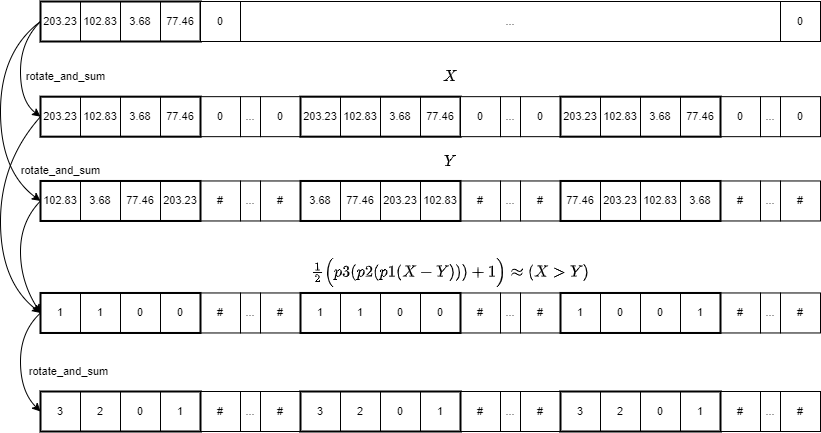
\includegraphics[width=0.8\textwidth]{array sorting figures/fig_1.png}
            \caption{A toy example illustrating the computation of sorted indices for an input array of size 4.}
            \label{fig:sorting-1}
        \end{figure}
        
        To perform the comparison, we approximate the sign function using a composite polynomial approach as described in \cite{Lee2021}. Specifically, three polynomials of degree 63 are used to approximate the function within the range $[-255, -0.01] \cup [0.01, 255]$ to satisfy the challenge requirements. Figure 2 shows the approximation, with a maximum absolute error below 0.0001. Polynomial evaluations are made using the baby step giant step (BSGS) algorithm \cite{Bossuat2021} to optimize level consumption. The comparison circuit utilizes 19 levels in total $(1+3\lceil \log_{2}63 \rceil)$, including an additional level for input value scaling. After applying the comparison function, rotation and summation operations are performed to accumulate results and compute the target indices (Figure 1).
        
        \begin{figure}[H]
            \centering
            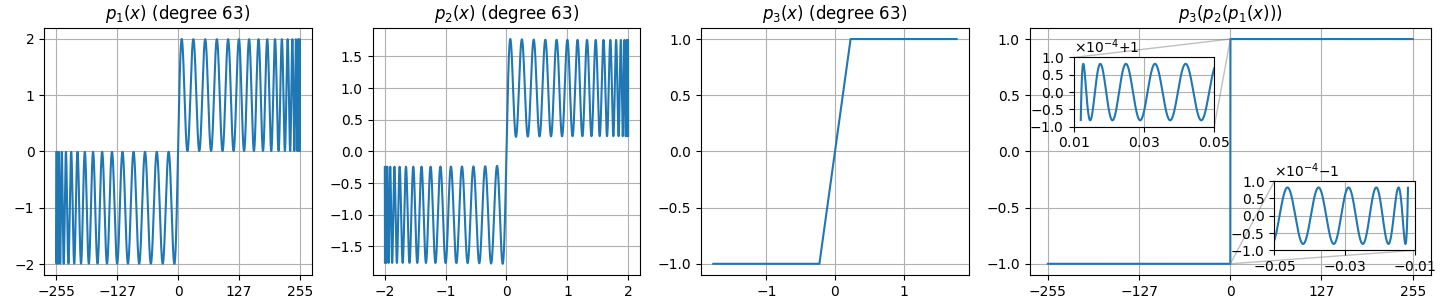
\includegraphics[width=0.8\textwidth]{array sorting figures/fig_2.png}
            \caption{Approximation of the sign function using a composition of three polynomials $p_1, p_2, p_3$ of degree 63.}
            \label{fig:sorting-2}
        \end{figure}
    
    \item \textbf{Permutation}:
    A permutation matrix is derived based on the computed indices, as demonstrated in Figure 6. This process requires an approximated equality-checking function, which is constructed as a composition of two polynomials with degrees 59 and 62, as shown in Figure 7. The array is then rearranged into sorted order using vector-matrix multiplication with the permutation matrix. This step consumes a total of 14 levels, obtained by $(\lceil \log_{2}59 \rceil + \lceil \log_{2}62 \rceil + 2)$,  where the additional two levels account for multiplication with the permutation matrix and a masking operation.

    \FloatBarrier % Forces all pending floats before this point
    \begin{figure}[H]
        \centering
        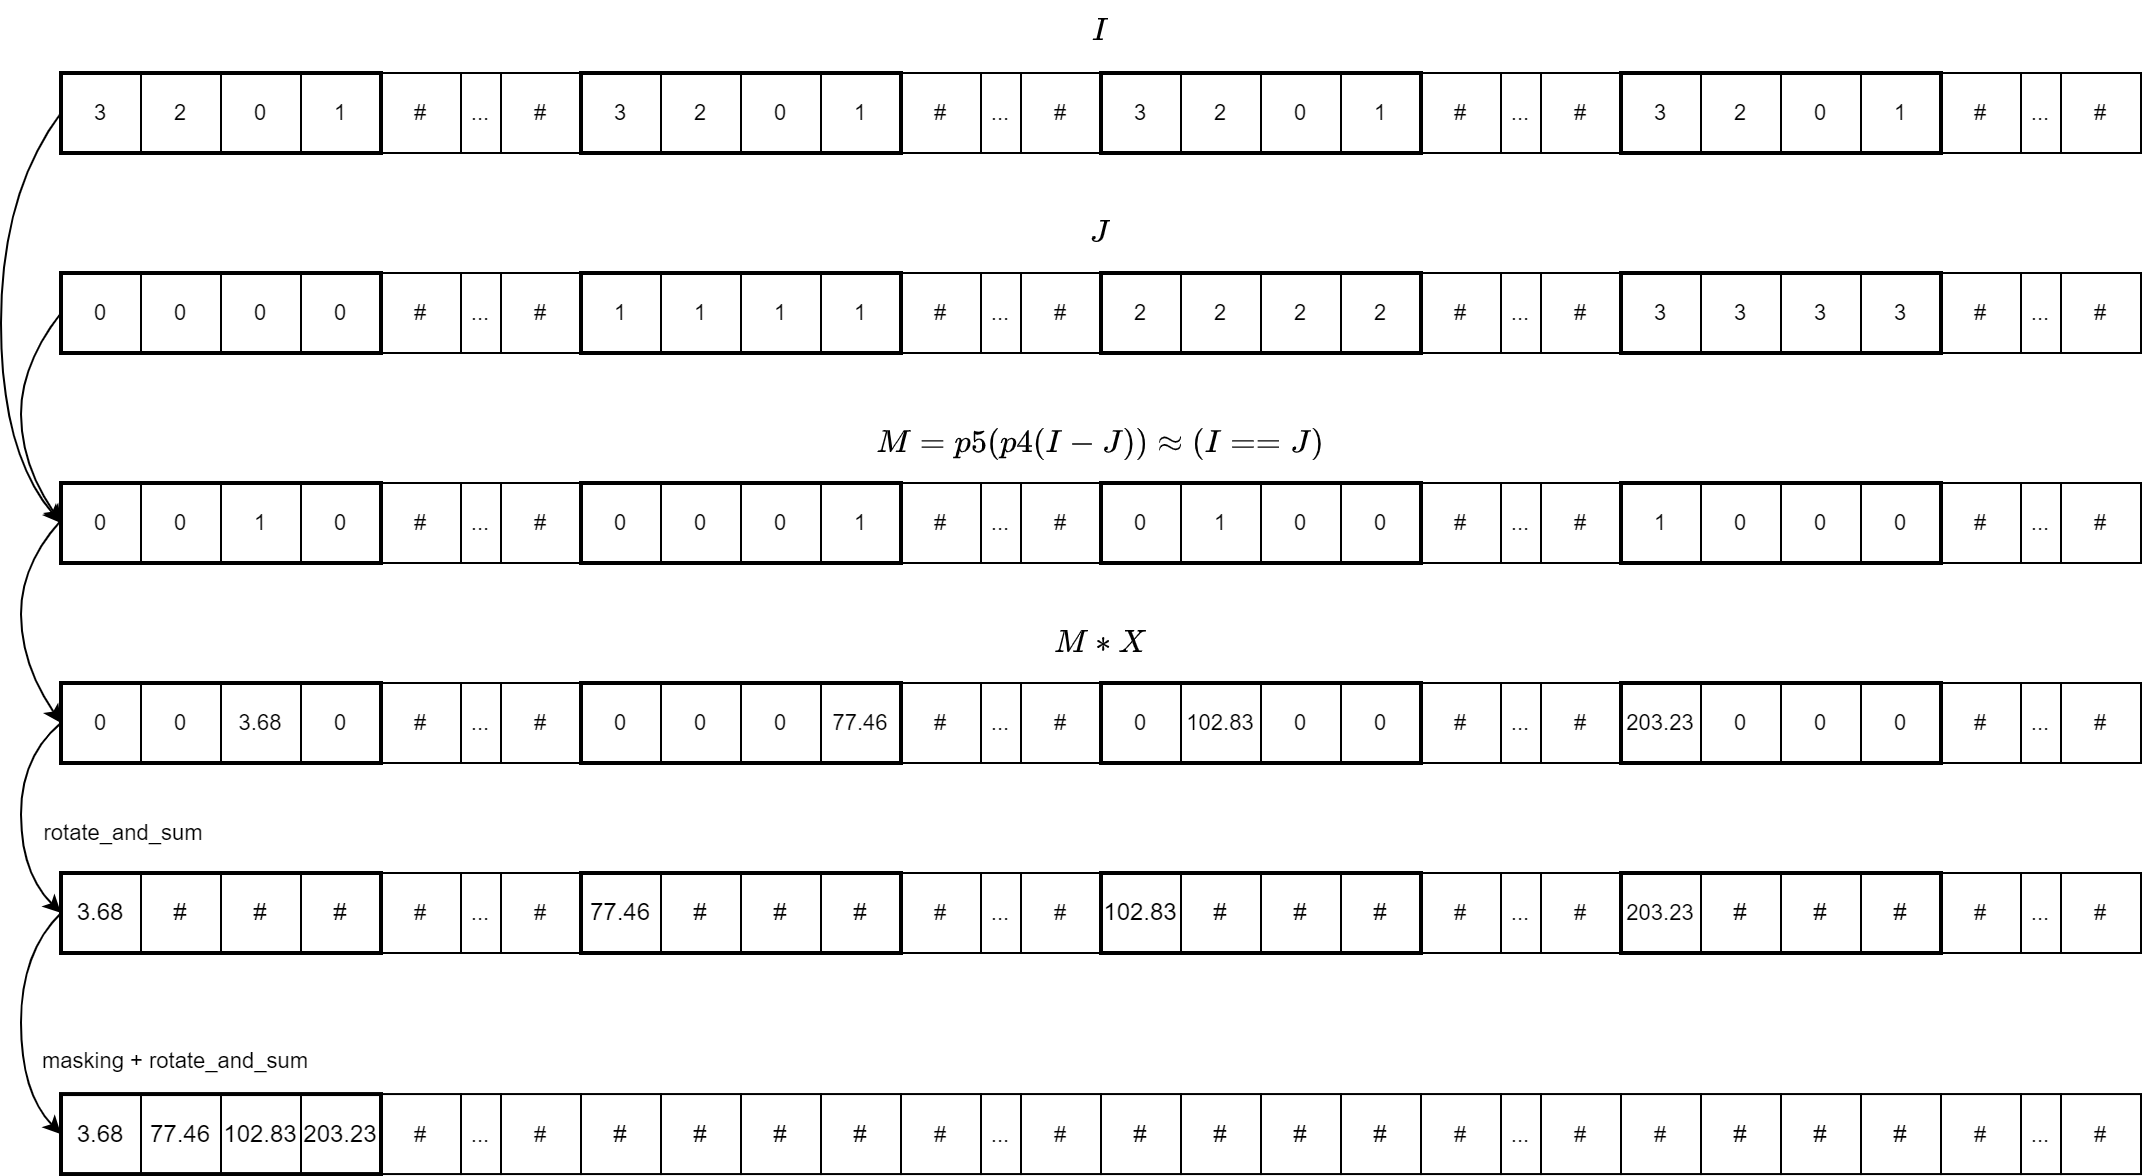
\includegraphics[width=0.8\textwidth]{array sorting figures/fig_3.png}
        \caption{Computation of the permutation matrix from the indices, followed by the rearrangement of array elements into sorted order.}
        \label{fig:sorting-3}
    \end{figure}
    
    \begin{figure}[H]
        \centering
        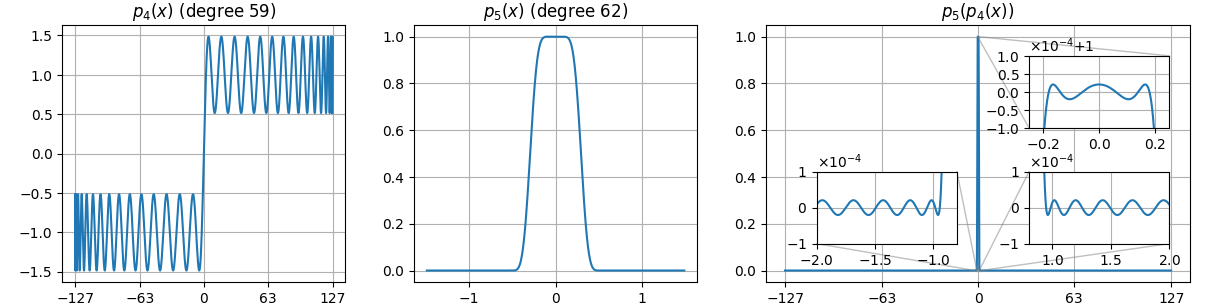
\includegraphics[width=0.8\textwidth]{array sorting figures/fig_4.png}
        \caption{Approximation of the equality checking function using a composition of three polynomials $p_4, p_5$ of degree 59 and 62}
        \label{fig:sorting-4}
    \end{figure}
    \FloatBarrier % Optional: Ensures no floats escape this section
\end{enumerate}
    


    \subsubsection{Max element}
The objective of the challenge is to find a maximum value in a vector encrypted under BFV.

\paragraph{Specification}
 \begin{itemize}
    \item \textbf{Input}: 
        \begin{itemize}
            \item encrypted vector A of size  2048, where each element is in range $[0, 255]$
            \item cryptocontext
            \item public key
            \item multiplication key
        \end{itemize}
    \item \textbf{Output}
        \begin{itemize}
            \item a ciphertext with maximum value
        \end{itemize}
    \item \textbf{Encryption parameters}:
        \begin{itemize}
            \item Number of slots: $2^{11}$ 
            \item Ring dimension: 16384
        \end{itemize}
\end{itemize}

     
\paragraph{Algorithm overview}\mbox{}\\

\begin{enumerate}
    \item \textbf{Comparison}. We use Lagrange interpolation to construct a polynomial that acts as a step function: $ f_i(x) = 
    \begin{cases} 1 & \text{if } x \geq i \\ 0 & \text{otherwise} 
    \end{cases} $
    
    \item \textbf{Threshold iteration}. Iterate over threshold values \( i = 1 \) to \( m = 255 \). For each \( i \), we evaluate whether each encrypted array element is greater than or equal to \( i \), so for each \( i \) there is an array of 0 and 1 (1 if $x_i \geq i$, 0 otherwise.)
    
    \item \textbf{Homomorphic NAND}. For each array obtained from the previous step we calculate if there's  any 1 in this array: 1 if yes, no otherwise
        \begin{lstlisting}
        def NAND(y, n):
            z = 1 - y
            r = 1
            while r < n:
                z = z * (z << r)
                r *= 2
            z = 1 - z
            return z
        \end{lstlisting}
        
    \item \textbf{Answer}. The maximum element is the sum of all NAND function results from previous step. The whole function pseudocode is
        \begin{lstlisting}
        def max(x, m=256):
            sum = 0
            for i in range(1, m):
                y = (x >= i)
                if np.any(y):
                    sum += 1
            return sum
        \end{lstlisting}

    \item \textbf{SIMD Parallelization}. Since $n = 2048$ is smaller than half the ring dimension (16384), we can duplicate the encrypted array across the available slots and process different thresholds (i) in parallel. The polynomial coefficients for each threshold are encoded as plaintext vectors, and ciphertext-plaintext multiplications are used to evaluate the different polynomials.
\end{enumerate}

\textbf{Example Use Case}:
\begin{itemize}
    \item In audio or sensor signals, finding the maximum amplitude is crucial for normalization, peak detection, or thresholding.
    \item In classification problems (like image recognition), the output layer gives multiple scores (e.g., for cat, dog, car), and the maximum score determines the predicted class.
    \item In max-pooling layers in CNNs (Convolutional Neural Networks), the maximum value in a region is used to reduce dimensionality while preserving strong signals.
\end{itemize}

\section{Privacy-Preserving AI Applications}

\subsection{Image Classification (CIFAR-10)}

\textbf{Image recognition} is a key task in machine learning and computer vision, where models are trained to identify and classify objects or patterns within images. By integrating fully homomorphic encryption (FHE), image recognition can be applied to sensitive data without compromising privacy, making it suitable for domains such as medical diagnostics, biometric identification, and surveillance systems.\\
In this challenge, the CIFAR-10 dataset is used, comprising 60,000 images distributed across 10 distinct classes. CIFAR-10 is widely recognized as a benchmark for assessing the performance of image classification models. Solution accuracy is evaluated as the percentage of correctly classified images.

\begin{itemize}
    \item \textbf{Task}: Multiclass classification
    \item \textbf{Dataset}: CIFAR-10
    \item \textbf{Evaluation Metric}:
        \begin{itemize}
            \item \textbf{Accuracy:} The percentage of correctly classified images.
        \end{itemize}
    \item \textbf{Formal Specification}: 
        \begin{itemize}
            \item \textbf{Input}: Encrypted vector \(x = (x_1, \ldots, x_{3072})\), where \(x_i \in [0,255]\)
            \item \textbf{Output}: Encrypted vector \(y=(y_1, ..., y_{10})\), where the index of the maximum element indicates the predicted class of the input image.
        \end{itemize}
\end{itemize}
 
\subsubsection{Solution 1: Encrypted Image Classification Using KAN}

\begin{itemize}
    \item \textbf{Architecture}: Kolmogorov-Arnold Network (KAN)
    \item \textbf{Encryption parameters}: 
        \begin{itemize}
            % \item Number of slots: 10
            \item Multiplication depth: 5
            \item Ring dimension: 8192
            \item Scale mod size: 25
            \item First mod size: 30
            \item Batch size: 4096
            \item Bootstrapping: unused
        \end{itemize}
    \item \textbf{Library}: OpenFHE \cite{OpenFHE}
    \item \textbf{Performance}: 
        \begin{itemize}
            \item Accuracy: 100\%
            \item Average inference time: 0.321 s/image
        \end{itemize}
\end{itemize}

\paragraph{Model Selection}\mbox{}

We experimented with various neural network architectures and eventually decided to use the Kolmogorov-Arnold Network (KAN) \cite{liu2025kankolmogorovarnoldnetworks}. Compared to traditional multilayer perceptron networks, KAN requires fewer model parameters and performs well in signal/function regression or interpolation tasks, making it well-suited for this challenge. To enhance evaluation efficiency, we adopted a variant of KAN based on Chebyshev polynomials, known as ChebyKAN \cite{ChebyKAN}. The Chebyshev basis can be efficiently computed using recursive formulas, thereby reducing computational costs and minimizing ciphertext level consumption.

\paragraph{Model Training}\mbox{}

We trained a KAN network with a single layer of learnable activation functions. To optimize runtime, we sought the lowest possible activation degree that could still achieve 100\% prediction accuracy. The training code was adapted from a GitHub repository \cite{ChebyKAN}. We successfully trained the model to a degree of 8, which required a multiplication depth of 5: one for normalizing the input vector and four for evaluating the Chebyshev polynomials.

\paragraph{Optimization}\mbox{}

Given that the input vector consists of 3,072 elements (from a 32x32 image with three channels), the minimum ring dimension we could use in the challenge was 8,192, with up to 4,096 plaintext slots to encrypt the entire input vector. We aimed to work with this lowest ring dimension to minimize complexity and maximize computation speed. We observed that the dominant HE operator during inference was the rotation operator, which necessitates costly key-switching calculations. Theoretically, to compute the sum over a vector of $N$ elements packed in a single ciphertext, one must perform $log⁡_2(N)$ rotations using the folding technique. With an input dimension of 3,072 and an output dimension of 10 classes, the first layer's forward pass (calculating 10 different summations for the 10 classes) would require at least $\left\lceil log⁡_2(3,072)\right\rceil+10−1=21$ rotations at a ring dimension of 8,192. To reduce this number and expedite the inference process, our idea is to infer the probability for each output class based on subsampled portions of the input image.

Specifically, the output probability for the $i$-th class was computed from pixels located at indices $i+10j$ where $j=0,1,…,306$, in the flattened input vector, as illustrated in Figure \ref{fig:pixel-selection}. In this manner, the output probability of a class can be viewed as a function interpolation task over approximately 307 pixels of the input image. Calculating the sum over these subsets of evenly-spaced pixels can be optimally achieved using $\left\lceil log⁡_2(307)\right\rceil =9$ rotations in total.
\begin{figure}[H]
    \centering
    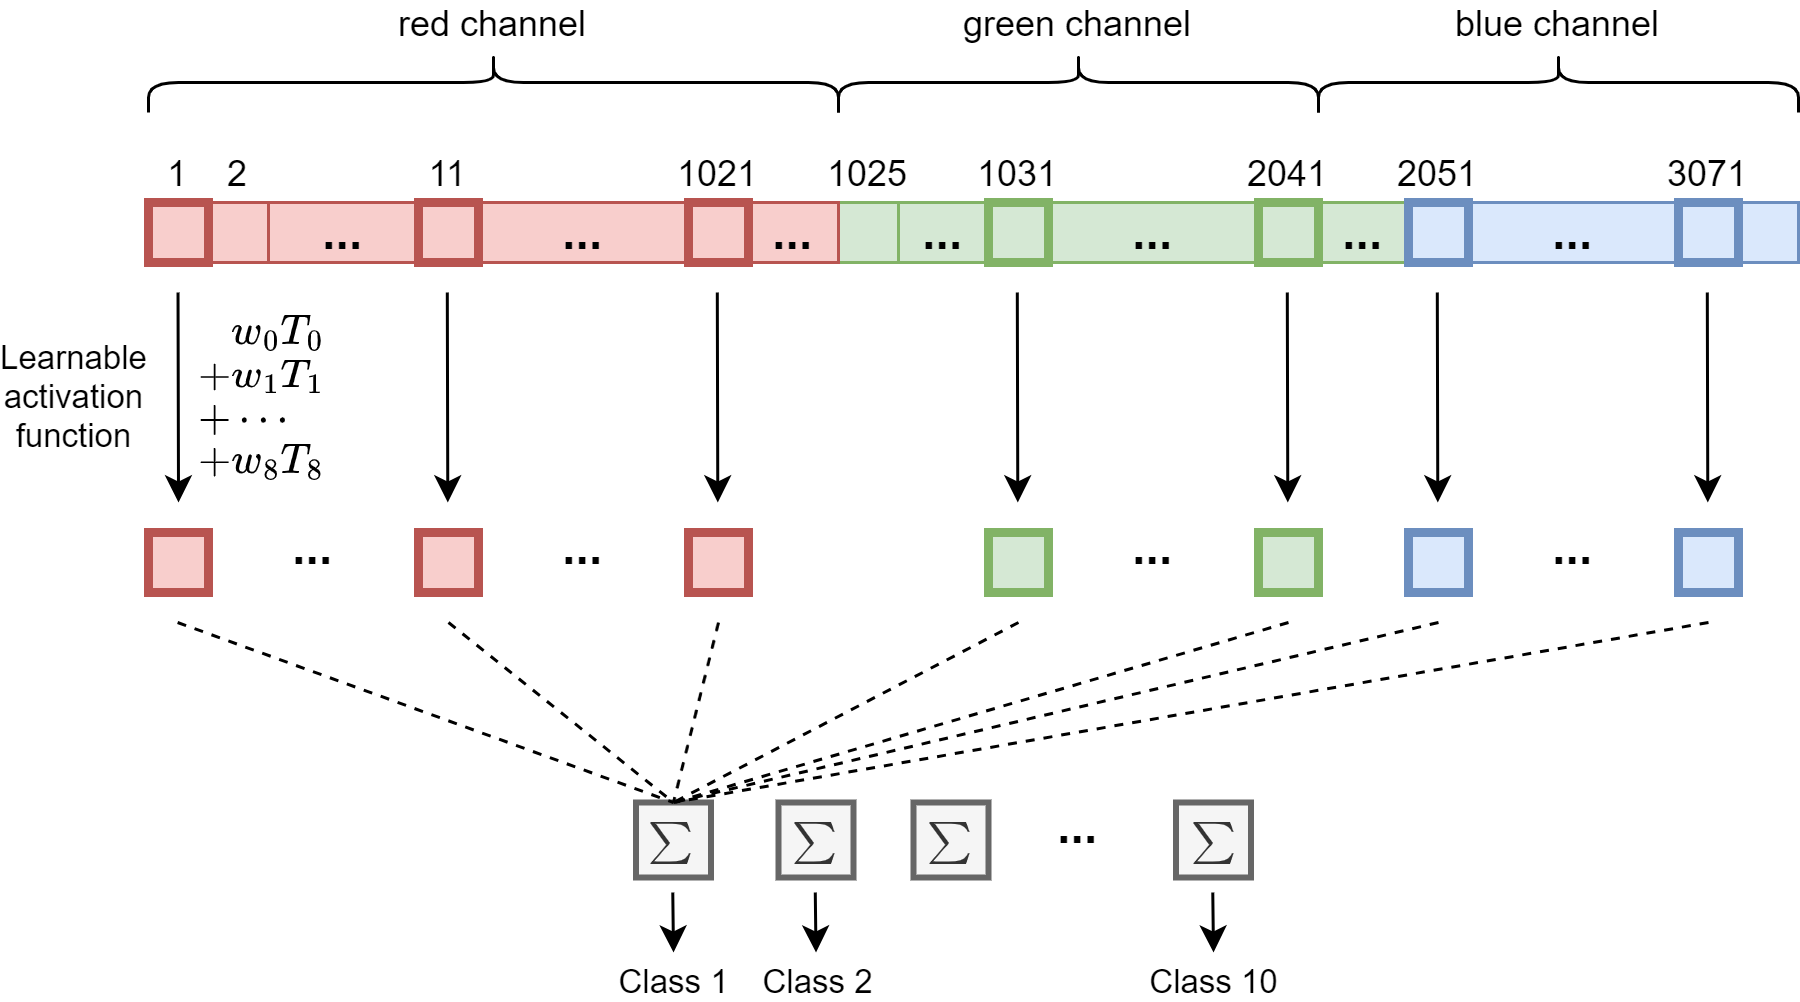
\includegraphics[width=1\linewidth]{figures_cifar/pixel_selection.png}
    \caption{Pixel selection for efficient class probability computation.}
    \label{fig:pixel-selection}    
\end{figure}

However, reducing the number of input dimensions also decreases accuracy, potentially falling below the acceptable threshold. To counteract this, we used multiple fragmented pixels at different offsets to predict class probabilities. Specifically, the probability for the $i$-th class was associated with pixels at positions $i+10j+offset$, with $j=0,1,\dots,306$ and $offset=0,\dots,n_{offset}$ (Figure \ref{fig:pixel-selection2}). A higher $n_{offset}$ results in higher prediction accuracy. By experimentally varying $n_{offset}$, we selected the lowest value yielding over 85\% accuracy, which was $n_{offset} = 3$ for the time-oriented track, and the lowest value achieving 100\% accuracy, which was $n_{offset} = 5$ for the accuracy-oriented track. Consequently, the number of rotation operations required for each track was $\left\lceil log⁡_2(3 \times 307) \right\rceil+3-1=12$ and $ \left \lceil log_{⁡2}(5 \times 307) \right \rceil+5-1=15$, respectively. By minimizing the number of required rotations, our approach significantly accelerates processing speed compared to other solutions that operate on the full image.
\begin{figure}[H]
 \centering
 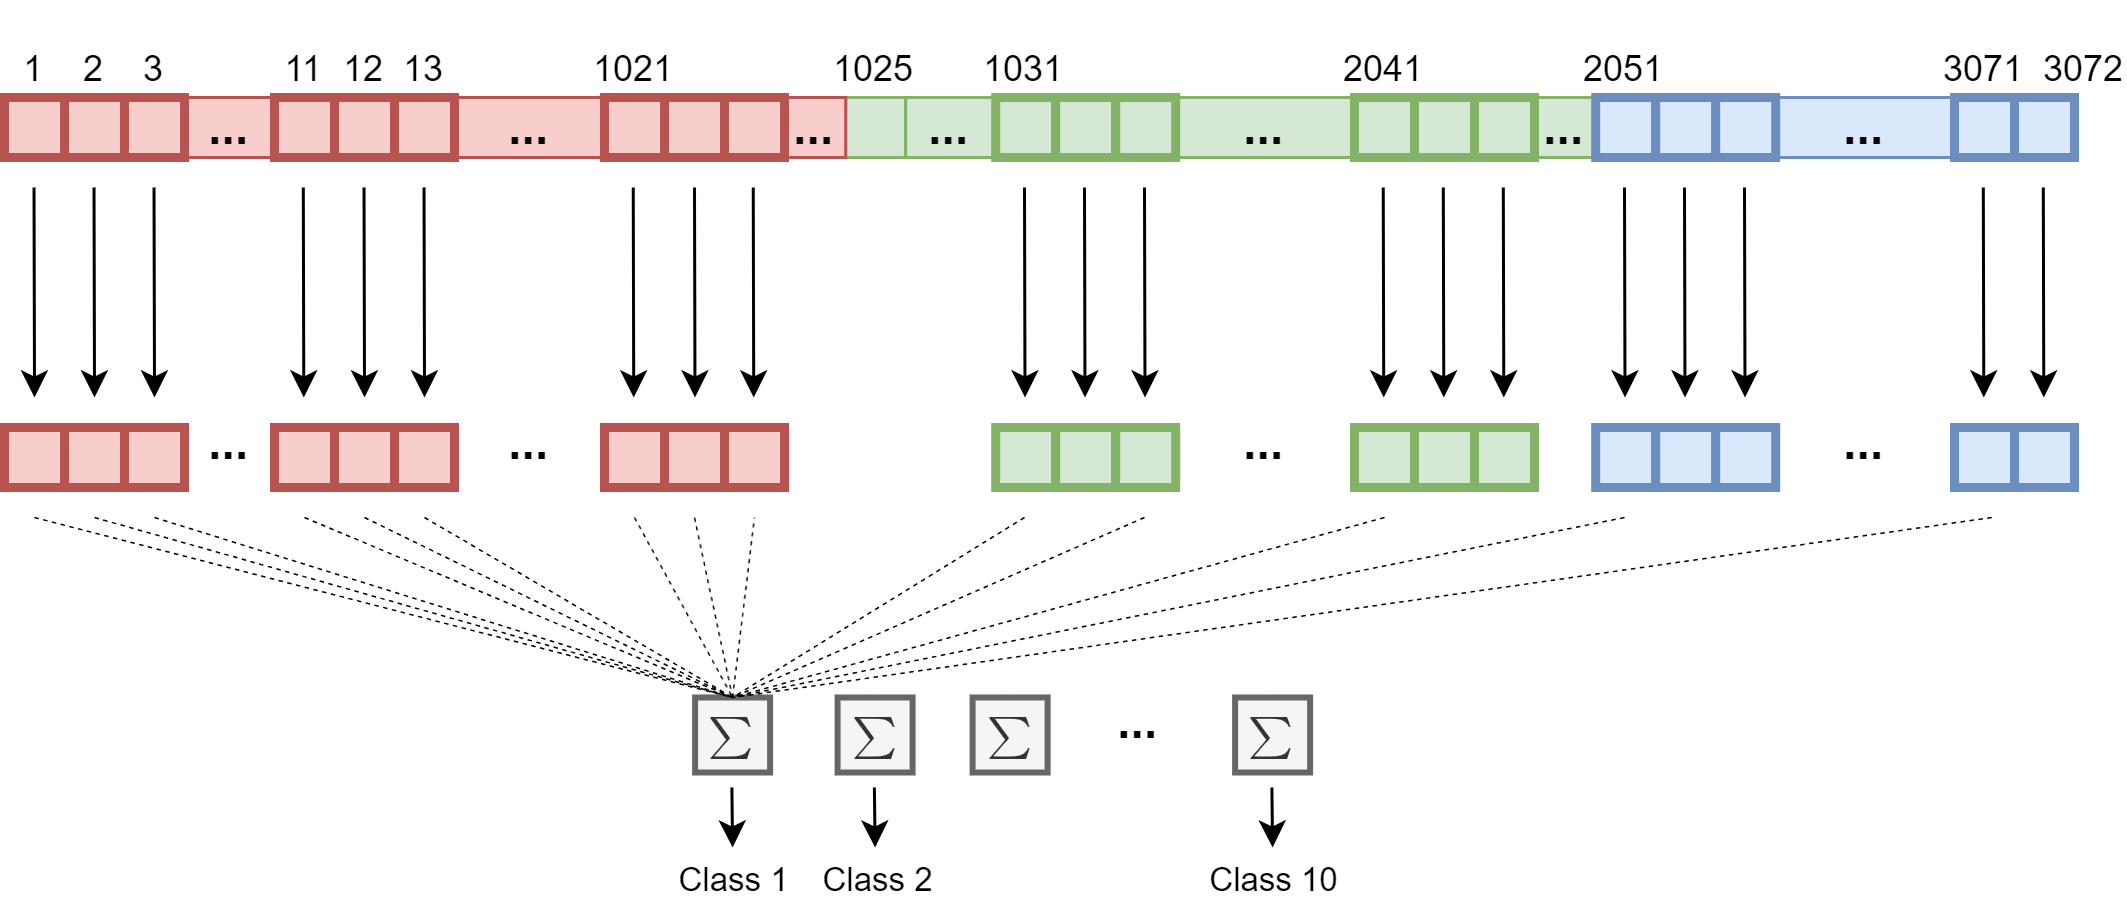
\includegraphics[width=1\linewidth]{figures_cifar/pixel_selection_2.png}
 \caption{Pixel selection with different offsets $n_{offset} = 3$ for enhanced class probability computation.}
 \label{fig:pixel-selection2}
\end{figure}

\subsubsection{Solution 2: Encrypted Image Classification Using MLP}

\begin{itemize}
    \item \textbf{Architecture}: Multilayer perceptron (MLP)
    \item \textbf{Encryption parameters}: 
        \begin{itemize}
            % \item Number of slots: 10
            \item Multiplication depth: 4
            \item Ring dimension: 16384
            \item Scale mod size: 51
            \item First mod size: 60
            \item Batch size: 4096
            \item Bootstrapping: unused
        \end{itemize}
    \item \textbf{Library}: LattiGo \cite{lattigo}
    \item \textbf{Performance}: 
        \begin{itemize}
            \item Accuracy: 100\%
            \item Average inference time: 0.236 s/image
        \end{itemize}
\end{itemize}

\paragraph{Model Selection}\mbox{}\\

Initially, we experimented with the ResNet architecture, however, given the nature of this particular challenge, we opted for a significantly simpler neural network model with one hidden layer. The chosen neural network model had the following architecture:

\begin{itemize}
    \item \textbf{Input Layer}: 3072 neurons (corresponding to the \verb|32x32x3| CIFAR-10 images).
    \item \textbf{Hidden Layer}: 16 neurons.
    \item \textbf{Output Layer}: 10 neurons (one for each CIFAR-10 class).
\end{itemize}
This configuration resulted in approximately 50000 parameters.


\paragraph{Model Training}\mbox{}\\


To achieve 100\% accuracy, we trained the model in two phases, each time using a different activation function to avoid local minimum issues:

\begin{enumerate}
    \item During the \textbf{first training phase}, we used a cubic activation function to improve neural network convergence.
    \item On the \textbf{second phase}, we continued training with a quadratic activation function. This allowed us to reduce the multiplication depth and, therefore, speed up the calculations.
\end{enumerate}
The training was conducted using the \verb|PyTorch| library. Training with the cubic activation function took one day, followed by two additional days of training with the quadratic activation function.

\paragraph{Loss function and optimizer}\mbox{}\\

We utilized cross-entropy as our loss function and the L-BFGS optimizer for training.

\begin{itemize}
    \item \textbf{Cross-entropy}, also known as logarithmic loss or log loss, is widely used in classification problems to measure the performance of a model.
    \item \textbf{L-BFGS} is a quasi-Newton method that approximates the algorithm of Broyden–Fletcher–Goldfarb–Shanno (BFGS) using limited computer memory. It iteratively improves an estimate of the inverse Hessian matrix and uses it to compute search directions.
\end{itemize}
These choices were made based on their compatibility with the nature of our problem and demonstrated higher accuracy with faster convergence compared to gradient methods.

\paragraph{Model deployment}\mbox{}\\

The model weights were exported in JSON format for use in the Go solution.

\paragraph{Operations on encrypted data}\mbox{}\\

Given the encrypted nature of the data, certain operations had to be implemented manually because the EvalSum key had not been generated:

\begin{itemize}
    \item \textbf{EvalSum} - custom implementation since sum keys were not provided.
    \item \textbf{DotProduct} - custom implementation of EvalInnerProduct was necessary for encrypted matrix multiplication.
\end{itemize}

\paragraph{Optimizations}\mbox{}\\

Normally, neural networks parallelize well, but Python's pickle serialization limitations hindered initial attempts to accelerate computations through parallelism. However, employing goroutines in Go and the LattiGo library, we managed to speed up execution by at least three times.

Additionally, we had to fix a few bugs in the code and implement unit, integration, and performance tests to be able to compare solutions efficiently.

Eventually, we reduced the number of multiplications, adjusted the parameters \verb|log_q| and \verb|log_n|, applied parallelism in Go, and managed to accelerate performance by additional 30\%.

\paragraph{Conclusion}\mbox{}\\

While our prototype demonstrates the feasibility of performing inference over encrypted data, the simplicity of the network architecture may limit its generalization capacity. Initial results suggest a risk of overfitting to the training data, which can be addressed through using deeper network, different activation functions and more extensive training.
 
\subsection{Fraud Detection}

\textbf{Fraud detection} plays a crucial role in ensuring financial security. FHE enables sensitive transaction data analysis without ever exposing it, preserving privacy throughout the process.

Participants are challenged to implement a Support Vector Machine (SVM) - a classic yet highly effective algorithm for classification tasks. The model must perform inference directly on encrypted transaction data, accurately determining whether each transaction is legitimate or fraudulent.

The overall accuracy of each solution is primarily evaluated using the F1 score, with both precision and recall considered in the final assessment.


\begin{itemize}
    \item \textbf{Task}: Binary classification
    \item \textbf{Dataset}: Ethereum Fraud Detection Dataset
    \item \textbf{Algorithm}: Support Vector Machine (SVM)
    \item \textbf{Evaluation Metrics:}
        \begin{itemize}
            \item \textbf{Recall}: The proportion of actual fraudulent transactions correctly identified by the model.
            \item \textbf{Precision}: The proportion of transactions classified as fraudulent that are truly fraudulent.
            \item \textbf{F1 Score}: The harmonic mean of precision and recall, providing a balanced measure of model performance when both false positives and false negatives are important.
        \end{itemize}
    \item \textbf{Formal Specification}: 
        \begin{itemize}
            \item \textbf{Input}: Encrypted vector $x = (x_1, ..., x_{45})$
            \item \textbf{Output}: Encrypted vector containing the result of transaction evaluations, where: 
                \begin{itemize}
                    \item \verb|-1| represents a legitimate transaction.
                    \item \verb|1| represents a fraudulent transaction.
                \end{itemize}
        \end{itemize}
\end{itemize}

\subsubsection{Solution 1: Fraud Detection via SVM with Linear Kernel}

\begin{itemize}
    \item \textbf{Encryption parameters}: 
        \begin{itemize}
            % \item Number of slots: 1 \ahmad{Please double-check this value, is it 1?}
            \item Multiplication depth: 26
            \item Ring dimension: 65536
            \item Scale mod size: 40
            \item First mod size: 45
            \item Batch size: 32768
            \item Bootstrapping: unused
        \end{itemize}
    \item \textbf{Library}: OpenFHE \cite{OpenFHE}
    \item \textbf{Performance}: 
        \begin{itemize}
            \item Accuracy: 91.3\%
            \item Average inference time: 12.761 s/transaction
        \end{itemize}
\end{itemize}


\paragraph{Data Preprocessing}\mbox{}\\

The public training dataset contains Ethereum transaction features for fraud detection. We analyzed feature skewness using \texttt{scipy.stats.skew}, revealing high skewness (>1) across all columns, indicating non-normal distributions.

\begin{lstlisting}
                                               Column   Skewness
0                                  ERC20 avg val sent  88.696538
1                                  ERC20 max val sent  88.682094
2                                  ERC20 min val sent  88.679603
3                                   ERC20 max val rec  88.631605
4                          ERC20 total Ether received  88.608206
...
36  total transactions (including tnx to create co...   6.797555
37            Time Diff between first and last (Mins)   1.802201
\end{lstlisting}

High skewness suggests that features are heavily tailed, which can degrade SVM performance by causing numerical instability or poor separation of classes. Transforming features to a logarithmic scale reduces skewness, making the data more symmetric and closer to a normal distribution. This ultimately boosts classification accuracy.

Since the dataset includes negative values, we first apply \texttt{MinMaxScaler} to scale features to [0, 1], then use a polynomial approximation of the logarithm (\texttt{poly\_log}) to enable HE-compatible evaluation.

\begin{lstlisting}
scaler = MinMaxScaler()
X_train = scaler.fit_transform(X_train)
X_test = scaler.transform(X_test)
X_train = poly_log(X_train)
X_test = poly_log(X_test)
\end{lstlisting}

The \texttt{poly\_log} function approximates the logarithm over [0.0001, 1] (figure \ref{fig:log-approximation}) using Chebyshev interpolation with degree 121 for high precision:

\begin{lstlisting}
x = np.linspace(0.0001, 1, 10000)
y = np.log(x)
poly_log = C.Chebyshev.fit(x, y, 121)
\end{lstlisting}

After log transformation, we apply a second \texttt{MinMaxScaler} to rescale the data back to [0, 1].

\begin{lstlisting}
scaler2 = MinMaxScaler()
X_train = scaler2.fit_transform(X_train)
X_test = scaler2.transform(X_test)
\end{lstlisting}

\begin{figure}
    \centering
    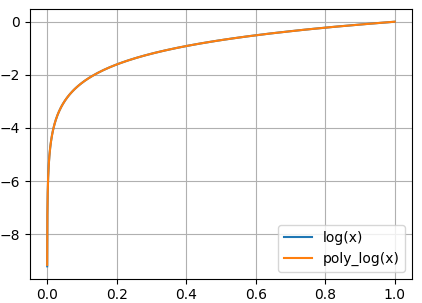
\includegraphics[width=0.5\linewidth]{figures_fraud_detection/log_approximation.png}
    \caption{Illustration of the log approximation.}
    \label{fig:log-approximation}
\end{figure}

\paragraph{Model Training}\mbox{}\\

We implemented SVM using \texttt{sklearn.svm.SVC} and tune hyperparameters \texttt{C} and \texttt{gamma} with GridSearchCV.

\begin{lstlisting}[language=Python]
tuned_parameters = [{ "gamma": [1,0.1,0.01,0.001], "C": [1, 10, 100, 1000]}]
grid = GridSearchCV(SVC(kernel='linear'), tuned_parameters, refit=True, cv=5, scoring='f1')
grid.fit(X_train, y_train)
\end{lstlisting}

We selected the linear kernel for its simplicity and HE compatibility. Non-linear kernels (e.g., RBF, polynomial) could improve accuracy but introduce significant complexity in HE. They require evaluating the kernel function over potentially hundreds of support vectors, involving costly operations like rotations. In contrast, the linear kernel’s decision function is a single dot product between the input vector and the model’s weights, enabling faster and more efficient HE inference.

The grid search yields an F1 score of 0.9025 on the training set. Validation on a separate clear-text test set achieves an F1 score of 0.9161, confirming robust generalization.

\begin{lstlisting}
print("Train F1 Score :",grid.best_score_)
best_y_pr = grid.predict(X_test)
print('Test F1 Score: ', f1_score(y_test, best_y_pr))
    
Output:
Train F1 Score : 0.9025388783902716
Test F1 Score:  0.9161290322580645
\end{lstlisting}

\paragraph{HE Implementation}\mbox{}\\

For HE inference, we use the CKKS scheme to evaluate the trained SVM on encrypted inputs. The process mirrors preprocessing and model evaluation in the clear-text domain but operates on ciphertexts.

First, we apply the \texttt{MinMaxScaler} and \texttt{poly\_log} transformation to the input ciphertext:

\begin{lstlisting}
// Extract attributes from the first MinMaxScaler, where scale_1 = scaler.scale_ and min_1 = scaler.min_
m_OutputC = m_cc->EvalMult(m_OutputC, m_cc->MakeCKKSPackedPlaintext(scale_1));
m_cc->EvalAddInPlace(m_OutputC, m_cc->MakeCKKSPackedPlaintext(min_1));
    
m_OutputC = m_cc->EvalChebyshevSeries(m_OutputC, poly_cheb, 0.0001, 1);
    
// Similarly, we have scale_2 = scaler2.scale_ and min_2 = scaler2.min_
// However, this second scaling can be skipped as discussed below
// m_OutputC = m_cc->EvalMult(m_OutputC, m_cc->MakeCKKSPackedPlaintext(scale_2));
// m_cc->EvalAddInPlace(m_OutputC, m_cc->MakeCKKSPackedPlaintext(min_2));
\end{lstlisting}

To optimize, we skip the second scaling (\texttt{scaler2}) by fusing it with the SVM weight multiplication, reducing the multiplication depth. We adjust the model weights and bias accordingly:

\begin{lstlisting}
w = grid.best_estimator_.coef_[0]
b = grid.best_estimator_.intercept_[0] + (scaler2.min_ * w).sum()
w = w * scaler2.scale_
\end{lstlisting}

The HE evaluation computes the decision function as a dot product:

\begin{lstlisting}
m_OutputC = m_cc->EvalMult(m_OutputC, m_cc->MakeCKKSPackedPlaintext(w));
int k = 64;
while (k > 1) {
    k = k/2;
    m_OutputC = m_cc->EvalAdd(m_OutputC, m_cc->EvalRotate(m_OutputC, k));
}
m_OutputC = m_cc->EvalAdd(m_OutputC, b);
\end{lstlisting}

This accumulates the dot product result in the first slot of the ciphertext. To obtain the predicted label, we compute the sign of this value. We scale the first slot to [-1, 1], mask other slots containing dummy values to avoid overflow, and apply an approximated sign function using three composite polynomials (each degree 25):

\begin{lstlisting}
std::vector<double> mask(32768);
mask[0] = 0.01; // Scale to [-1, 1]
m_OutputC = m_cc->EvalMult(m_OutputC, m_cc->MakeCKKSPackedPlaintext(mask));
    
m_OutputC = m_cc->EvalChebyshevSeries(m_OutputC, sign_poly_1, -1, 1);
m_OutputC = m_cc->EvalChebyshevSeries(m_OutputC, sign_poly_2, -1, 1);
m_OutputC = m_cc->EvalChebyshevSeries(m_OutputC, sign_poly_3, -1, 1);
\end{lstlisting}

This produces the final encrypted classification label (1 for fraud, -1 for legitimate).

\paragraph{Conclusion}\mbox{}\\

The solution achieves high accuracy (F1 > 0.91) on the Ethereum fraud detection task while enabling secure inference on encrypted data with a processing delay of 12.761 seconds per inference. By leveraging a linear SVM, Chebyshev polynomial approximations, and optimized HE operations, we balance performance and computational efficiency.

\subsubsection{Solution 2: Fraud Detection via SVM with RBF Kernel}

\begin{itemize}
    \item \textbf{Encryption parameters}: 
        \begin{itemize}
            % \item Number of slots: 1
            \item Multiplication depth: 25
            \item Ring dimension: 65536
            \item Batch size: 32768
            \item Bootstrapping: unused
        \end{itemize}
    \item \textbf{Library}: OpenFHE \cite{OpenFHE}
    \item \textbf{Performance}: 
        \begin{itemize}
            \item Accuracy: 90.2\%
            \item Average inference time: 39.378 s/transaction
        \end{itemize}
\end{itemize}


\paragraph{Data Preprocessing}\mbox{}\\

For fraud detection on Ethereum transactions, a Support Vector Machine (SVM) with a Radial Basis Function (RBF) kernel was selected due to its superior performance in capturing complex, non-linear patterns in transaction data. The RBF kernel is defined as:
\[
K(x, x_i) = \exp\left(-\gamma \lVert x - x_i \rVert^2\right)
\]

\textbf{Optimal Hyperparameters}
\begin{itemize}
    \item Kernel coefficient (\texttt{gamma}): 0.5
    \item Regularization (\texttt{C}): 1200
    \item Number of support vectors: 512
\end{itemize}

This configuration resulted in the highest observed F1-score. Despite the numerous features and support vectors, the SIMD (Single Instruction, Multiple Data) capabilities of CKKS homomorphic encryption ensured minimal computational overhead.

\paragraph{Homomorphic Inference}\mbox{}\\
The SVM decision function is computed as:
\[
f(x) = \operatorname{sign} \left( \sum_{i=1}^{n} y_i \, K(x, x_i) + b \right)
\]
Where:
\begin{itemize}
    \item The Ethereum transaction feature vector x is \textbf{encrypted}
    \item Support vectors ($x_i$), dual coeffs ($y_i$) and bias ($b$) are in \textbf{clear}
\end{itemize}


\paragraph{Key Challenges \& Solutions}\mbox{}\\
\begin{itemize}
    \item Non-Polynomial Kernel Approximation
        \begin{itemize}
            \item The RBF kernel is non-polynomial and cannot be directly evaluated in CKKS.
            \item \textbf{Solution:} A polynomial approximation over the interval $[-30000, 0]$ with a degree-1024 polynomial was employed to ensure high precision.
        \end{itemize}
    \item Sign Function Approximation
        \begin{itemize}
            \item The sign function is discontinuous and must be approximated in encrypted computation.
            \item \textbf{Practical approximation:} Polynomial approximation of the hyperbolic tangent ($tanh$) approximation with:
                \begin{itemize}
                    \item \textbf{Polynomial Degree:} 256
                    \item \textbf{Approximation Interval:} $[-70, 70]$
                    \item \textbf{Sharpness Parameter ($\alpha$):} 6 (higher $\alpha$ improves the approximation to the sign function but must be chosen carefully with respect to the degree)
                \end{itemize}
        \end{itemize}
    \item Efficient SIMD Packing
        \begin{itemize}
            \item SIMD batching allows to parallelize kernel evaluations, significantly reducing latency in encrypted inference. Specifically, the 64 features of the 512 support vectors can fit int $64\times512=32684$ slots, taking full advantage of the available plaintext capacity. Each block of 64 slots computed the kernel between the encrypted transaction and a support vector. 
        \end{itemize}
\end{itemize}

\paragraph{SIMD Inference Steps}\mbox{}\\

The following steps outline how SIMD operations are leveraged to perform efficient homomorphic inference:
\begin{itemize}
    \item SIMD squaring of feature differences
    \item Local summation to compute squared distances
    \item Kernel evaluation for each computed distance
    \item SIMD multiplication of kernels with dual coefficients
    \item Global summation across relevant slots, followed by bias addition
    \item Homomorphic sign approximation for the final prediction
\end{itemize}

\paragraph{Implementation with OpenFHE}\mbox{}\\

All polynomial approximations and evaluations were performed using the OpenFHE library’s EvalChebyshevFunction method. The approximation intervals were selected taking into account the outputs of the decision function on the training dataset.

\subsection{House Price Prediction}

Accurately predicting housing prices is essential in real estate, benefiting everyone from individual buyers to large-scale investors. However, real-world datasets often include sensitive information, raising privacy concerns.

This challenge invites participants to build a regression model for estimating housing prices using Fully Homomorphic Encryption (FHE). 

The overall quality of the solutions is primarily assessed by the R-squared score, with both MAE and MSE also considered in the final assessment.  

\begin{itemize}
    \item \textbf{Task}: Regression
    \item \textbf{Dataset}: California Housing Prices
    \item \textbf{Evaluation Metric}:
        \begin{itemize}
            \item \textbf{Mean Absolute Error (MAE)}: calculates the average difference between the calculated values and actual values. It shows how far the model’s prediction from the true house price.
            \item \textbf{Mean Squared Error (MSE)}: the average squared difference between the estimated values and true value. The MSE incorporates both the variance of the estimator and its bias.
            \item \textbf{R-squared (Coefficient of Determination)}: the proportion of variation in the dependent variable (y) that is accounted for by the regression line, compared to the variation explained by the mean of y. Essentially, it measures how much more accurately the regression line predicts each point’s value compared to simply using the average value of y.
        \end{itemize}
    \item \textbf{Formal Specification}: 
        \begin{itemize}
            \item \textbf{Input}: Encrypted vector \(x = (x_1, ..., x_{13})\)
            \item \textbf{Output}: Encrypted model prediction indicating the resulted price
        \end{itemize}
\end{itemize}

\subsubsection{Solution: House Price Prediction Using KAN}

\begin{itemize}
    \item \textbf{Architecture}: Kolmogorov-Arnold Network (KAN)
    \item \textbf{Encryption parameters}: 
        \begin{itemize}
            % \item Number of slots: 1
            \item Multiplication depth: 13
            \item Ring dimension: 32768
            \item Scale mod size: 40
            \item First mod size: 60
            \item Batch size: 16384
            \item Bootstrapping: unused
        \end{itemize}
    \item \textbf{Library}: OpenFHE \cite{OpenFHE}
    \item \textbf{Performance}: 
        \begin{itemize}
            \item Accuracy: 85.051\%
            \item Average inference time: 2.401 s/record
        \end{itemize}
\end{itemize}

\paragraph{Model Selection}\mbox{}\\

We selected the Kolmogorov-Arnold Network (KAN) \cite{liu2025kankolmogorovarnoldnetworks} for its efficiency in regression tasks and its compact architecture, which requires fewer parameters than conventional neural networks such as multilayer perceptrons. Specifically, we adopted a Chebyshev polynomial-based variant known as ChebyKAN \cite{ChebyKAN}, which replaces the original spline-based activations in KAN with Chebyshev polynomials. This substitution not only preserves the expressive power of the model but also ensures compatibility with HE schemes. Chebyshev polynomials can be evaluated efficiently using recursive relations and are well-suited for encrypted computation, as they avoid the complexities introduced by spline interpolation. As a result, ChebyKAN significantly reduces both computational overhead and ciphertext level consumption, making it ideal for privacy-preserving inference under HE.

\paragraph{Model Architecture}\mbox{}\\

The ChebyKAN model used is a two-layer neural network implemented in PyTorch, with each layer incorporating Chebyshev polynomial operations for non-linear regression.

\begin{itemize}
    \item \textbf{Input Normalization:} A min-max scaler maps input features to the range [-0.8, 0.8] (instead of the standard [-1, 1]) to provide a safety margin, preventing overflow when processing unseen test samples during encrypted inference.
    \item \textbf{First Layer:} Transforms the normalized inputs into a hidden representation by computing weighted sums of Chebyshev polynomials.
    \item \textbf{Activation:} Applies a scaled hyperbolic tangent activation ($0.9tanh⁡(⋅)$) to constrain outputs within [-0.9, 0.9], ensuring numerical stability and preventing overflow.
    \item \textbf{Second Layer:} Aggregates the hidden representations to generate the final price prediction using Chebyshev-based polynomial transformation.
\end{itemize}

\paragraph{Model Training}\mbox{}\\

Training procedures were adapted from an open-source implementation \cite{ChebyKAN}. We conducted a grid search over the polynomial degrees and hidden layer sizes to maximize performance, measured by the R2 score on a validation set. The best configuration identified through this process used a hidden dimension of 32 and a Chebyshev polynomial degree of 7.

\paragraph{Model Ensembling}\mbox{}\\

To improve prediction robustness and accuracy, we trained multiple ChebyKAN models with different random initializations and combined their output using an ensemble approach. Predictions from individual models were aggregated through a weighted combination, with the weights optimized via the L-BFGS-B algorithm to maximize the ensemble’s R2 score. This ensemble strategy mitigates model variance and achieves superior predictive performance compared to any single model.

\paragraph{HE Inference}\mbox{}\\

For encrypted inference, we customized the Baby-Step Giant-Step (BSGS) algorithm to efficiently evaluate Chebyshev polynomials on encrypted data. By using plaintext coefficient vectors and SIMD evalutation, our modified BSGS approach enables simultaneous evaluations of multiple polynomials across different inputs. The method requires only three multiplicative levels to evaluate Chebyshev polynomials of degree 7, minimizing the depth required for inference.

\subsection{k-Nearest Neighbors Search}
k-nearest neighbors (kNN) search is used in many AI applications, including recommendation systems, semantic search, retrieval-augmented generation (RAG) systems, etc. The main idea is to find the most similar entities (products, documents, vectors) to a given query. 

This challenge invites participants to implement a k-nearest neighbors algorithm for encrypted two-dimensional vectors using cosine similarity. The input vector is encrypted, while dataset containing the target vectors is not encrypted. The task is to enable kNN search ensuring the privacy of the query vector and the retrieved nearest neighbors.

The accuracy of the solution is evaluated using  recall@10.


\begin{itemize}
    \item \textbf{Task}: Vector search
    \item \textbf{Dataset}: 2D vectors
    \item \textbf{Evaluation Metric}:
        \begin{itemize}
            \item \textbf{Recall@10}: the percentage of the true ten nearest neighbors that were correctly retrieved by the solution. 
        \end{itemize}
    \item \textbf{Formal Specification}: 
        \begin{itemize}
            \item \textbf{Input}: Encrypted vector $x = (x_1, x_{2})$
            \item \textbf{Output}: Encrypted vector containing ten nearest neighbors 
        \end{itemize}
\end{itemize}

\subsubsection{Solution: Encrypted Cosine Similarity}

\begin{itemize}
    \item \textbf{Similarity metric}: Cosine similarity
    \item \textbf{Encryption parameters}: 
        \begin{itemize}
            % \item Number of slots: 10
            \item Multiplication depth: 100
            \item Ring dimension: 65536
            \item Scale mod size: 44
            \item First mod size: 60
            \item Batch size: 32768
            \item Levels available after bootstrap: 6
        \end{itemize}
    \item \textbf{Library}: OpenFHE \cite{OpenFHE}
    \item \textbf{Performance}: 
        \begin{itemize}
            \item Accuracy: 100\%
            \item Average inference time: 20.523 s/query
        \end{itemize}
\end{itemize}

\paragraph{Introduction}\mbox{}\\

The challenge tasks players with finding the $k$ nearest neighbors of an encrypted 2D vector within a database, using cosine similarity to measure the distance between vectors. Cosine similarity is defined as $d(\mathbf{u}, \mathbf{v}) = 1 - \frac{\mathbf{u} \cdot \mathbf{v}}{|\mathbf{u}| |\mathbf{v}|}$, where $\mathbf{u}$ and $\mathbf{v}$ are vectors, $\cdot$ denotes the dot product, and $|\cdot|$ represents the Euclidean norm. A common approach to find $k$-nearest neighbors (kNN) in cleartext is to compute the cosine similarity between the query vector and all database vectors, sort the similarities in descending order, and select the top $k$ vectors. This can be optimized using data structures like KD-trees or approximate methods like locality-sensitive hashing for efficiency.

However, a naive implementation of such an algorithm in the HE domain may incur significant overhead due to the high computational cost of encrypted arithmetic operations, the need for deep circuits to evaluate non-linear functions like division and square roots in cosine similarity, limited support for comparison and sorting operations, and the increased ciphertext size and noise growth in HE schemes.

\paragraph{Approach}\mbox{}\\

We adopted an approximated approach that simplifies the kNN problem into a lookup table. This is based on the observation that two vectors are likely to share similar neighbors if the angle between them is small. In particular, we partition the 2D plane into $M$ uniform angular sectors, defined by a set of $M$ vectors ${\mathbf{v}_0, \mathbf{v}_1, \dots, \mathbf{v}_{M-1}}$, where each $\mathbf{v}_i$ is equally spaced at angles $\frac{2\pi i}{M}$ from the origin. Here, the $i$-th sector is the sector between $\mathbf{v}_{i-1}$ and $\mathbf{v}_i$. The neighbor set of a sector is defined as the $k$ nearest neighbors of its bisector ray, precomputed during initialization. For a query vector $\mathbf{x}$, we identify the sector it falls into by computing its angle relative to the origin and return the precomputed neighbors of that sector as its approximate neighbors. Figure \ref{fig:angular-section} illustrates this partitioning approach.

\begin{figure}
    \centering
    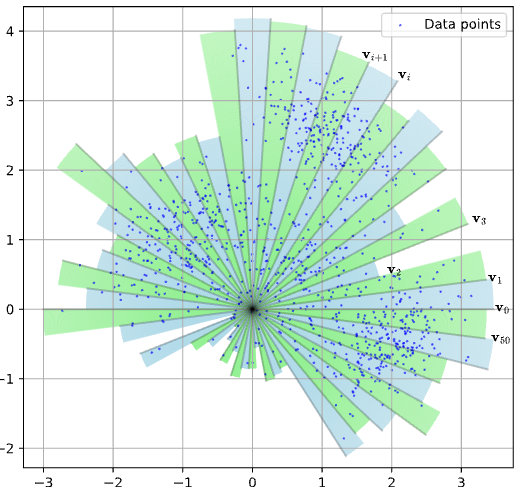
\includegraphics[width=0.5\linewidth]{figures_knn/angular_section.png}
    \caption{Illustration of the angular sector partitioning approach with $M=50$ sectors.}
    \label{fig:angular-section}
\end{figure}
Given a 2D query vector $\mathbf{x}$, we can determine if it falls into the $i$-th sector by evaluating the dot products $\mathbf{x} \cdot \mathbf{v}_{i-1}$ and $\mathbf{x} \cdot \mathbf{v}_i$ and checking if these values have opposite signs. In the HE domain, this check can be translated to computing the product of the dot products, i.e., $(\mathbf{x} \cdot \mathbf{v}_{i-1}) \cdot (\mathbf{x} \cdot \mathbf{v}_i) = (x[0]v_{i-1}[0] + x[1]v_{i-1}[1]) * (x[0]v_i[0] + x[1]v_i[1])$, using basic HE operations. We then apply an approximation of the sign function to the result to check if the value is negative, confirming sector membership.

It's straightforward that the accuracy of the prediction increases as the number of sectors increases, though this comes at the cost of higher computational requirements. At a very large number of clusters, the accuracy approaches perfection, but the computational cost may become excessively high. However, given the nonuniform distribution of data points, we can employ a nonuniform clustering approach to reduce the number of clusters. This involves denser partitioning in directions with more points and coarser partitioning in less populated areas. Specifically, we start with a high-resolution partition of $M=5000000$ clusters, which achieves perfect accuracy, and then gradually reduce the number of clusters by merging consecutive clusters that share the same set of $k$ nearest neighbors. This process is repeated until no further merging is possible, resulting in $M=1001$ clusters after the procedure, significantly reducing the computational overhead. Figure \ref{fig:angular_sectors2} shows an illustration of the resulting nonuniform partition. The high-level pseudocode for reducing the number of clusters is as follows:

\begin{lstlisting}
> For each sector:
>     Compute k nearest neighbors of the sector's center
>     Store the neighbor set in a map
> 
> Sort sectors in ascending order of start angle
> 
> Initialize an empty list for merged sectors
> While there are sectors to process:
>     Group consecutive sectors with the same k-NN set
>     Merge each group into a single sector
>     Add the merged sector to the list
> Update the sector list with the merged sectors
\end{lstlisting}

\begin{figure}
    \centering
    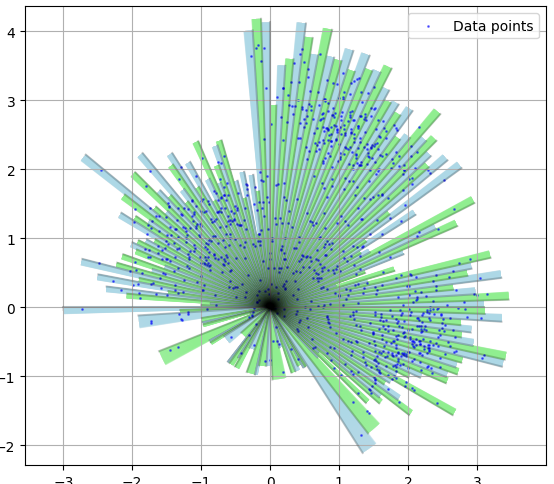
\includegraphics[width=0.5\linewidth]{figures_knn/angular_sectors.png}
    \caption{Illustration of the resulting nonuniform partition after merging clusters.}
    \label{fig:angular_sectors2}
\end{figure}

\paragraph{HE Implementation}\mbox{}\\

We now describe the HE implementation for determining the sector of a query vector $\mathbf{x}$ and mapping it to the corresponding precomputed $k$ nearest neighbors, using the sector-based approximation approach. The process is broken down into multiple steps as follows.

\begin{itemize}
    \item \textbf{Step 0:}: The process starts with a ciphertext $\text{ct}_\mathbf{x}$ containing the 2D query vector $\mathbf{x} = [x[0], x[1]]$. The components $x[0]$ and $x[1]$ are placed in the first two slots of the ciphertext, with all subsequent slots set to zero.
    \item \textbf{Step 1: Replicate the query vector across slots}:  To enable simultaneous computation across multiple sectors, the query vector $\mathbf{x}$ is replicated across the ciphertext slots. After replication, each pair of slots in $\text{ct}_\mathbf{x}$ (e.g., slots 0–1, 2–3, etc.) contains the values $[x[0], x[1]]$.
    \item \textbf{Step 2: Make a plaintext for sector boundary vectors}: A plaintext $\text{pt}_\mathbf{v}$ is created to store the sector boundary vectors ${\mathbf{v}_0, \mathbf{v}_1, \dots, \mathbf{v}_M}$. For each sector $i$, the vector $\mathbf{v}_i$ is placed in specific slot pairs. For example, slots from $32i$ to $32i+31$ corresponding to sector $i$ will contain the replications of $[\mathbf{v}_i[0], \mathbf{v}_i[1]]$. This allows for the computation of dot products with consecutive sector boundaries.
    \item \textbf{Step 3: Compute dot products with sector boundaries}: For each sector $i$, the dot products $\mathbf{x} \cdot \mathbf{v}_{i-1}$ and $\mathbf{x} \cdot \mathbf{v}_i$ are computed in the HE domain. This involves element-wise subtraction between the replicated query vector and the sector boundary vectors, followed by rotation and multiplication. Specifically, the dot product $\mathbf{x} \cdot \mathbf{v}_i$ is calculated as $(\text{ct}_\mathbf{x}-\text{pt}_\mathbf{v})*\text{Rotate}(\text{ct}_\mathbf{x}-\text{pt}_\mathbf{v}, 1)$.
    \item \textbf{Step 4: Determine the sign of dot products}: To check if $\mathbf{x}$ lies between $\mathbf{v}_{i-1}$ and $\mathbf{v}_i$, we need to determine if the dot products $\mathbf{x} \cdot \mathbf{v}_{i-1}$ and $\mathbf{x} \cdot \mathbf{v}_i$ have opposite signs. An approximation of the sign function is evalutated over the dot product results using Paterson-Stockmeyer algorithm, converting the numerical dot products into boolean indicators (1 if the dot product is positive and 0 if negative).
    \item \textbf{Step 5: Identify sector}: The sector membership test relies on the fact that $\mathbf{x}$ lies in sector $i$ if $(\mathbf{x} \cdot \mathbf{v}_{i-1}) \cdot (\mathbf{x} \cdot \mathbf{v}_i) < 0$, indicating opposite signs. In the HE domain, this is implemented by multiplying the sign indicators of the two dot products. If the product is 1 (i.e., one sign is positive and the other negative), $\mathbf{x}$ is confirmed to be in sector $i$.
    \item \textbf{Step 6: Map to precomputed neighbors}: Once the sector of $\mathbf{x}$ is identified, the precomputed $k$ nearest neighbors associated with that sector are retrieved. These neighbors were calculated during the preprocessing phase for each sector's bisector ray. The neighbor sets are encoded into a single plaintext and is assigned to the slots corresponding to the identified sector by multiplication, ensuring that the output ciphertext only contains the approximate $k$ nearest neighbors of $\mathbf{x}$.
\end{itemize}

\section{Concluding remarks}

This paper presents the initial release of the FHERMA FHE Components library — a collection of fundamental operations and computational primitives designed for use within fully homomorphic encryption (FHE) frameworks. The current version reflects the collaborative efforts of a broader community, with the goal of systematizing and validating reusable building blocks for privacy-preserving computation.

As of this release, the component set includes representative examples from several key algorithmic domains, including linear algebra, non-linear transformations, sorting, and selection operations. These components are intended to serve both as implementation references and as a basis for further optimization and adaptation across various FHE schemes.

Future work will focus on several directions. First, we plan to incrementally extend the library with additional components, particularly those arising from concrete application demands in areas such as privacy-preserving machine learning and secure data analytics. Second, we intend to maintain regular updates to this document, incorporating community contributions and tracking improvements in performance, correctness, and generality of individual components. Third, we aim to improve the structure and modularity of the library in order to support its use as a foundation for higher-level algorithm design.

In the longer term, we envision the development of a structured reference — a ``cookbook'' — that formalizes patterns and practices in FHE algorithm construction. Such a reference would aim to support systematic reuse, reduce development overhead, and facilitate the integration of FHE into complex systems by providing well-defined, composable, and interoperable components.

The sustainability and evolution of this library will rely on continued community involvement, rigorous documentation, and a shared commitment to advancing the practical usability of FHE-based computation.

\printbibliography
\end{document}
